%\documentclass[letterpaper,conference]{IEEEtran}
\documentclass[a4paper,twocolumn,journal]{IEEEtran}
\usepackage{amsfonts,amssymb,amsmath}
\usepackage{epsfig,graphicx,color}
%\usepackage{subfigure}
\usepackage{url}
\usepackage{citesort}

% Example definitions.
% --------------------
\input ftw_macros.tex

\IEEEoverridecommandlockouts

\sloppy

%\addtolength{\textheight}{1.5cm}

\begin{document}

% Title.
% ------
\title{OpenAirInterface---An Experimental Platform for Next Generation Wireless Networks\thanks{Eurecom's Research is supported in part by its industrial partners: Swisscom, Thales, SFR, Orange France, Hitachi Europe, STMicroelectronics, Bouygues Telecom, Sharp, Cisco, BMW Group. This work is also funded in part by the European Commission through project CHORIST (ICT/FP6), the French National Research Agency (ANR) through projects AIRNET and HNPS, and by the  Wiener Wissenschafts-, Forschungs-und Technologiefonds (WWTF) through the project PUCCO. Parts of this work were presented at the COST2100 Workshop on MIMO and Cooperative Communications, June 2008, Trondheim, Norway.}}

% author names and affiliations
% use a multiple column layout for up to three different
% affiliations
\author{\IEEEauthorblockN{Florian Kaltenberger, Rizwan Ghaffar, Raymond Knopp, Hicham Anouar, Christian Bonnet}\\
\IEEEauthorblockA{Eurecom \\
 2229, Route des Cretes - B.P. 193\\
 06904 Sophia Antipolis, France\\
 Email (corresponding author): florian.kaltenberger@eurecom.fr}
}

\maketitle

\begin{abstract}


OpenAirInterface is an experimental open-source real-time hardware and software platform for experimentation in wireless communications and signal processing. Its current implementation provides a full software modem comprising physical and link layer functionalities for cellular and mesh network topologies. 

The physical (PHY) layer of the platform targets WiMAX and UMTS LTE like networks and thus uses MIMO-OFDMA as modulation and multiple access technique. The current hardware supports 5\,MHz bandwidth and two transmit/receive antennas. The media access (MAC) layer of the platform supports an abundant two-way signaling for enabling collaboration, scheduling protocols as well as traffic and channel measurements. 

%In order to maximize the system throughput, future wireless communication systems will employ a very tight frequency reuse. This causes scenarios with very high interference, expecially at the cell edges. The key ingredient to such networks are thus receiver structures that are able to deal with this interference.

In this paper we focus on the mesh topology and show how to implement a single-frequency fully-synchronized mesh network with OpenAirInterface. The key ingredient to enable such a network is a distributed MIMO receiver structure and a distributed network synchronization algorithm. We show how the distributed MIMO receiver is implemented in real-time on the OpenAirInterface platform. Further we provide results from field trails and compare them to the simulation results.


% In wirelss mesh networks nodes may cooperate to relay their information more efficiently to the destination. Such cooperative communication strategies however require tight interaction between physical, link and network layers.

% The platform is designed for a full software-radio implementation, in the sense that all protocol layers run on the host PCs under the control of a Linux real time operation system.

% Applications of the OpenAirMesh platform include demonstration of broadband ad hoc communications systems for public safety units as well as demonstration of collaborative communication in a cognitive radio system. In addition to the basic architecture of OpenAirMesh we will describe some field trials that were carried out in Barcelona, Spain.

\end{abstract}

%\tableofcontents


% activate the control type entry
%\bstctlcite{IEEEexample:BSTcontrol}

\section{Introduction}

% Motivation and contribution

The design and implementation of next generation wireless networks is a very challenging task. To ensure optimal performance it is necessary to carry out performance evaluations and field trials in parallel to standard development. Easily reconfigurable testbeds are a convenient way to investigate new ideas and to tackle many problems at an early development stage. This paper presents the Eurecom testbed OpenAirInterface, which is an experimental real-time, open-source hardware and software platform for future wireless networks. OpenAirInterface can be seen as a mock standard for realistic experimentation purposes which retains the salient features of a real radio system, without all the required mechanisms one would find in a standard used in deployment of commercial networks.

Apart from a general overview of OpenAirInterface, we report how it can be used to study some major challenges in future wireless networks. One such challenge is interference which is caused by a very tight frequency reuse in order to increase the network throughput. Interference is especially strong for users at the cell edge severely limiting the user's throughput. 

Most state-of-the-art wireless systems deal with the interference either by orthogonalizing the communication links in time or frequency \cite{Gesbert07adaption} or by allowing the communication links to share the same degrees of freedom but modeling the interference as additive Gaussian random process \cite{Russell1995}. Both of these approaches may be suboptimal as the first approach entails an \textit{a priori} loss of degrees of freedom in both links, no matter how weak the potential interference is while the second approach treats interference as pure noise while it actually carries information and has structure that can be potentially exploited in mitigating its effect. 

In \cite{ghaffar08b,ghaffar08c} a receiver structures that exploit the structure of the interference have been proposed. It was shown that exploiting the fact that the interference comes from a finite constellation alphabet, the information rate of the desired stream can be increased by up to one bit/sec/Hz. The same authors also derive a low-complexity max-log MAP receiver for these scenarios \cite{ghaffar09a}. In this paper we apply this kind of receiver to a distributed multiple-input multiple-output (MIMO) scenario, where one receiver is able to decode independent data streams from two different sources.

Another big challenge in future wireless networks is synchronization between nodes, especially indoors where a reference timing signal such as provided by the global positioning system (GPS) cannot be used. Synchronization is needed for example for the distributed MIMO receiver and to enable collaborative between base-stations both on the media access (MAC) and the physical (PHY) layer. 

In nature, distributed synchronization scheme can be observed on the flashing of fireflies \cite{Buck1976}. Recently, this nature-inspired scheme has been applied to synchronization in wireless networks \cite{simeone08distributed,tyrell06fireflies,hong05scalable,hu06scalability}. However, most of these works consider the isolated synchronization problem and neglecting the actual data communication. The pulse-coupled oscillator model (the model inspired by firefly synchronization) assumes that nodes have to be listening to all other nodes except during its own transmission of the synchronization pulse and immediately afterwards (refractory period). Therefore data transmission can only take place in the refractory period. However, this period must not be very long because otherwise the system becomes unstable \cite{hong05scalable}. 

In this paper we describe a more simple distributed time synchronization method and its implementation on the OpenAirInterface platform. It uses one node (the primary clusterhead) as a reference time clock. Nodes within the broadcast domain of the primary CH relay the synchronization signal, allowing other nodes to synchronize to the network. 

% idea: synch pulses are only tranmitted every x frames. However, timing drift might be too large between x frames -> simulate tradeoff

% another idea: synchronization is divided betweeen CH and MR. Both MR and CH transmit data after the pulse. The refractory period is appended after the TTI frame (this is when the pulse from the other part (MR or CH) is received).

% two examples: LTE-A and Mesh networks for civil protection
Synchronization and interference cancellation receivers can be readily applied to existing and future wireless networks. For example, in LTE-Advanced it is foreseen that many small base stations (so called femto base stations) are added to the network. These base stations might use the same frequency band as the macro cells, forming an overlay network. These femto base stations might also employ cooperative communications, i.e., a user might be connected to more than one femto base station or to a macro base station and a femto base station at the same time. Since femto base stations are usually employed indoors, they can only be synchronized by over the air communication. 

%Since these femto base stations might use an ADSL connection or even a wireless link to connect to the operators backbone network, no real-time signaling between them is possible.

% example 2
Another example where synchronization and interference cancellation is useful is a wireless mesh network (WMN). A WMN consist of a set of nodes, where each node operates not only as a host but also as a router, forwarding packets on behalf of other nodes that may not be within direct wireless transmission range of their destinations. A WMN is dynamically self-organized and self-configured, with the nodes in the network automatically establishing and maintaining mesh connectivity among themselves (creating, in effect, an ad hoc network) \cite{akyildiz05wireless}. WMNs can be used as rapidly-deployable broadband ad hoc communications systems for public safety units in interventions following natural hazards and industrial accidents. Such public safety units require a reliable communication broadband system and services that do not need heavy management operations involvement in order to allow them to increase their efficiency during their critical interventions.  
%Here the elements of the mesh network are routers, some of which are edge routers in the sense that they are gateways to other networks (WIFI, bluetooth, etc.).  These are some of the application scenarios considered in the CHORIST FP6 project (www.chorist.eu) and future HNPS Celtic project.

% WMNs can use cooperative transmission to greatly increase power efficiency, reliability and throughput. Such techniques refer to scenarios where one or more relay nodes are used to perform some type of distributed spatial processing technique, such as space-time coding \cite{Laneman2004a,Sendonaris2003} or distributed Hybrid-Automatic-Repeat-Request (HARQ) protocols \cite{azarian05,tabet07}. 


\paragraph*{Organization} 
Section \ref{sec:overview} gives an overview of the OpenAirInterface experimental platform. Section \ref{sec:architecture} presents the network, the link layer and the physical layer architecture of OpenAirMesh---a mesh network built using the OpenAirInterface. Section \ref{sec:ic} describes a novel low-complexity dual-stream receiver architecture used in OpenAirMesh. Finally we give show results from computer simulations as well as real experiments in Section \ref{sec:exp}. We conclude the paper in Section \ref{sec:con}. 

\paragraph*{Notation}
Let $\mathbb{C}$ denote the set of complex numbers. Scalars are denoted by $x$. Column vectors and matrices are denoted by $\Vec{a}$ and $\Mat{A}$ and their elements are denoted by $a_i$ and $A_{i,j}$ respectively. Transpose and Hermitian transpose are denoted by $\cdot^T$ and $\cdot^H$. $\Mat{I}_M$ is the identity matrix of size $M$ and $\Vec{0}_M$ is an $M$-dimensional vector of zeros. The Euclidean ($\ell_2$) norm of a vector $\Vec{a}$ is denoted by $\|\Vec{a}\|$ and the Frobenius norm of a matrix $\Mat{A}$ is denoted by $\|\Mat{A}\|_F$. $\mathbb{E}$ denotes expectation, and $\mathcal{CN}(\Vec{m},\Mat{C})$ denotes a multivariate proper complex normal distribution with mean vector $\Vec{m}$ and covariance matrix $\Mat{C}$.



\section{OpenAirInterface Overview}
\label{sec:overview}

The OpenAirInterface platform consists of both hardware and the software components. Additionally it comprises different simulation tools as well as collaborative web tools. The hardware components are described in subsection \ref{sec:hard}. In subsection \ref{sec:soft} we describe the basic organization of the OpenAirInterface software components (which are available under the GNU GPL from the OpenAirInterface website\footnote{\url{http://www.openairinterface.org}}). Finally we describe some related platform activities in Section \ref{sec:related}. 

\subsection{Hardware Components}
\label{sec:hard}

\begin{figure*}[t]
 \centering
 \includegraphics[height=5cm]{./figures/cbmimo.eps}
 \includegraphics[height=5cm]{./figures/expressMIMO.eps}
 \caption{CBMIMO1 and Express MIMO boards}
 \label{fig:hardware}
\end{figure*}

In OpenAirInterface there are two different hardware modules available: CardBus MIMO 1 (CBMIMO1) and it successor Express MIMO (cf.\ Figure \ref{fig:hardware}). All current activities (including the experiments described in this paper) are based on CBMIMO1. The Express MIMO hardware is already available and will be ready to use by the end of 2009. In the following we will describe the main characteristics of the two boards.

The CBMIMO1 board comprises two time-division duplex (TDD) radio frequency (RF) chains operating at 1.900-1.920 GHz with 5 MHz channels and 21dBM transmit power per antenna for an orthogonal frequency division modulated (OFDM) waveform\footnote{EURECOM has a frequency allocation for experimentation around its premises in Sophia Antipolis.}. As the name suggests in communicates with a host PC over the CardBus/PCMCIA interface. The cards house a medium-scale field programmable gate array (FPGA) (Xilinx X2CV3000) which makes use of the open-source LEON3 embedded processor from Geisler research. In the current version, the FPGA is mainly responsible for interfacing with with RF frontend as well as framing of the transmit and receive signals. All the PHY layer signal processing is usually run in real-time on the host PC under the control of the real-time application interface (RTAI), which is an extension to the  Linux operating system.

Express MIMO is a baseband processing board only providing significantly more processing power and bandwidth than CBMIMO1. It comprises two FPGAs: one Xilinx XC5VLX330 for real-time embedded signal processing applications and one Xilinx XC5VLX110T for control. Further employs for high-speed A/D and D/A converters from Analog Devices proving sampling rates up to 30.72 MHz (see \cite{Muhammad2008} for more details). A RF board for Express MIMO called Agile RF is also available. It offers significantly more RF functionality in terms tuning range and channel bandwidth than CBMIMO1. The tuning range per RF chain is 180MHz-8GHz with 20MHz channels. In addition, frequency division duplex (FDD) communication will also be possible. 

\subsection{Software Components}
\label{sec:soft}

The software components are organized into four areas (folders), which correspond more or less to the different layers of the Open Systems Interconnection (OSI) reference model. The areas also correspond to the directory structure on the OpenAirInterface Subversion (SVN) server.

\paragraph{openair0: Wireless Embedded System Design}
This folder mainly contains descriptions of the CBMIMO1 and Express MIMO hardware and the firmware for the corresponding FPGAs.  
\paragraph{openair1: Baseband signal processing}
This folder contains the code for the physical layer software modem along with RTAI/Linux device drivers and user-space tools to control the hardware. 
It also contains simulation environments and channel models to test the code without the hardware or to do performance simulations. Further, openair0 provides also the functionality for the Eurecom MIMO OpenAir Sounder (EMOS) to perform MIMO channel measurements over multiple users \cite{kaltenberger09}.
\paragraph{openair2: Medium-Access Protocols}
This folder contains the layer 2 protocol stack development for PCs along with Linux networking device drivers for Internet Protocol (IP) and Multiprotocol Label Switching (MPLS) interconnection.  This pertains to both cellular and mesh network topologies. The folder also contains an abstraction of the PHY layer, providing an efficient emulation platform for layer 2 and higher algorithms. 
\paragraph{openair3: Wireless Networking}
This contains the layer 3 protocol stack development for both all-IP cellular and IP/MPLS mesh networks. 

%\paragraph{Simulation Environments}


%\subsection{Collaborative Web Tools}

\subsection{Related Work}
\label{sec:related}


Testbeds for digital radio communications have become very popular, since they provide an effective mean to validate new ideas in an early development stage. Several testbeds with similar aims to OpenAirInterface exist, but only a few of them are open-source. Two such open-source platforms are the GNU radio project \cite{gnuradio} together with the Universal Software Radio Peripheral (USRP) from Ettus Research \cite{ettus} and the wireless open-access research platform (WARP) from Rice University \cite{warp}.

\subsubsection{GNU Radio}
The GNU radio is a collection of open-source libraries for all common software radio needs, including various modulations (GMSK, PSK, QAM, OFDM, etc.), error-correcting codes (Reed-Solomon, Viterbi, Turbo Codes), signal processing constructs (optimized filters, FFTs, equalizers, timing recovery), and scheduling. It allows applications to be developed in C++ or Python. The GNU software is easily configured with the USRP from Ettus Research, which consists of an FPGA, four AD/DA converters and slots for daughterboards for various RF frontends. The USRP is responsible only for data acquisition and transmission and the samples are transferred to and from the PC over USB or Gigabit Ethernet.

Compared to the OpenAirInterface platform, the GNU radio project does not provide a full reference design, but only building blocks. Further, a MAC layer implementation is missing in the current distribution. Also the USRP hardware has its limitations, mainly due to the connection to the PC over USB or Ethernet, which severely limits the achievable system throughput.

\subsubsection{WARP} 

The WARP platform consists of open-source hardware as well as software. The hardware comprises a motherboard with an FPGA that is responsible for the baseband processing. The motherboard can be extended with other processing boards and/or RF boards. The software library consists of platform support packages (low-level, PowerPC, and peripherals support), building blocks (synchronization, (de-)modulation, channel (de-)coding, ...) and reference designs  (for example an OFDM MIMO transceiver and a simple MAC layer). 

Like the OpenAirInterface, WARP is also a full software defined radio (SDR), but physical layer algorithms have to be developed either directly in VHDL or using the Xilinx System Generator toolchain for Matlab. Compared to the OpenAirInterface, this approach requires a steep learning curve and is very time consuming. Also, the Xilinx System Generator is not openly available.


\section{OpenAirMesh Architecture}
\label{sec:architecture}

In this section we present the specification and the implementation of OpenAirMesh---a mesh network built using the OpenAirInterface \cite{anouar08}. We start off by describing the network topology in Subsection \ref{sec:topology}. In Subsection \ref{sec:mac} we describe the layer 2 and finally in Subsection \ref{sec:phy} the physical layer. The last Subsection also contains a description of the network synchronization algorithm used in OpenAirMesh.

\subsection{Network Topology}
\label{sec:topology}

\begin{figure*}
 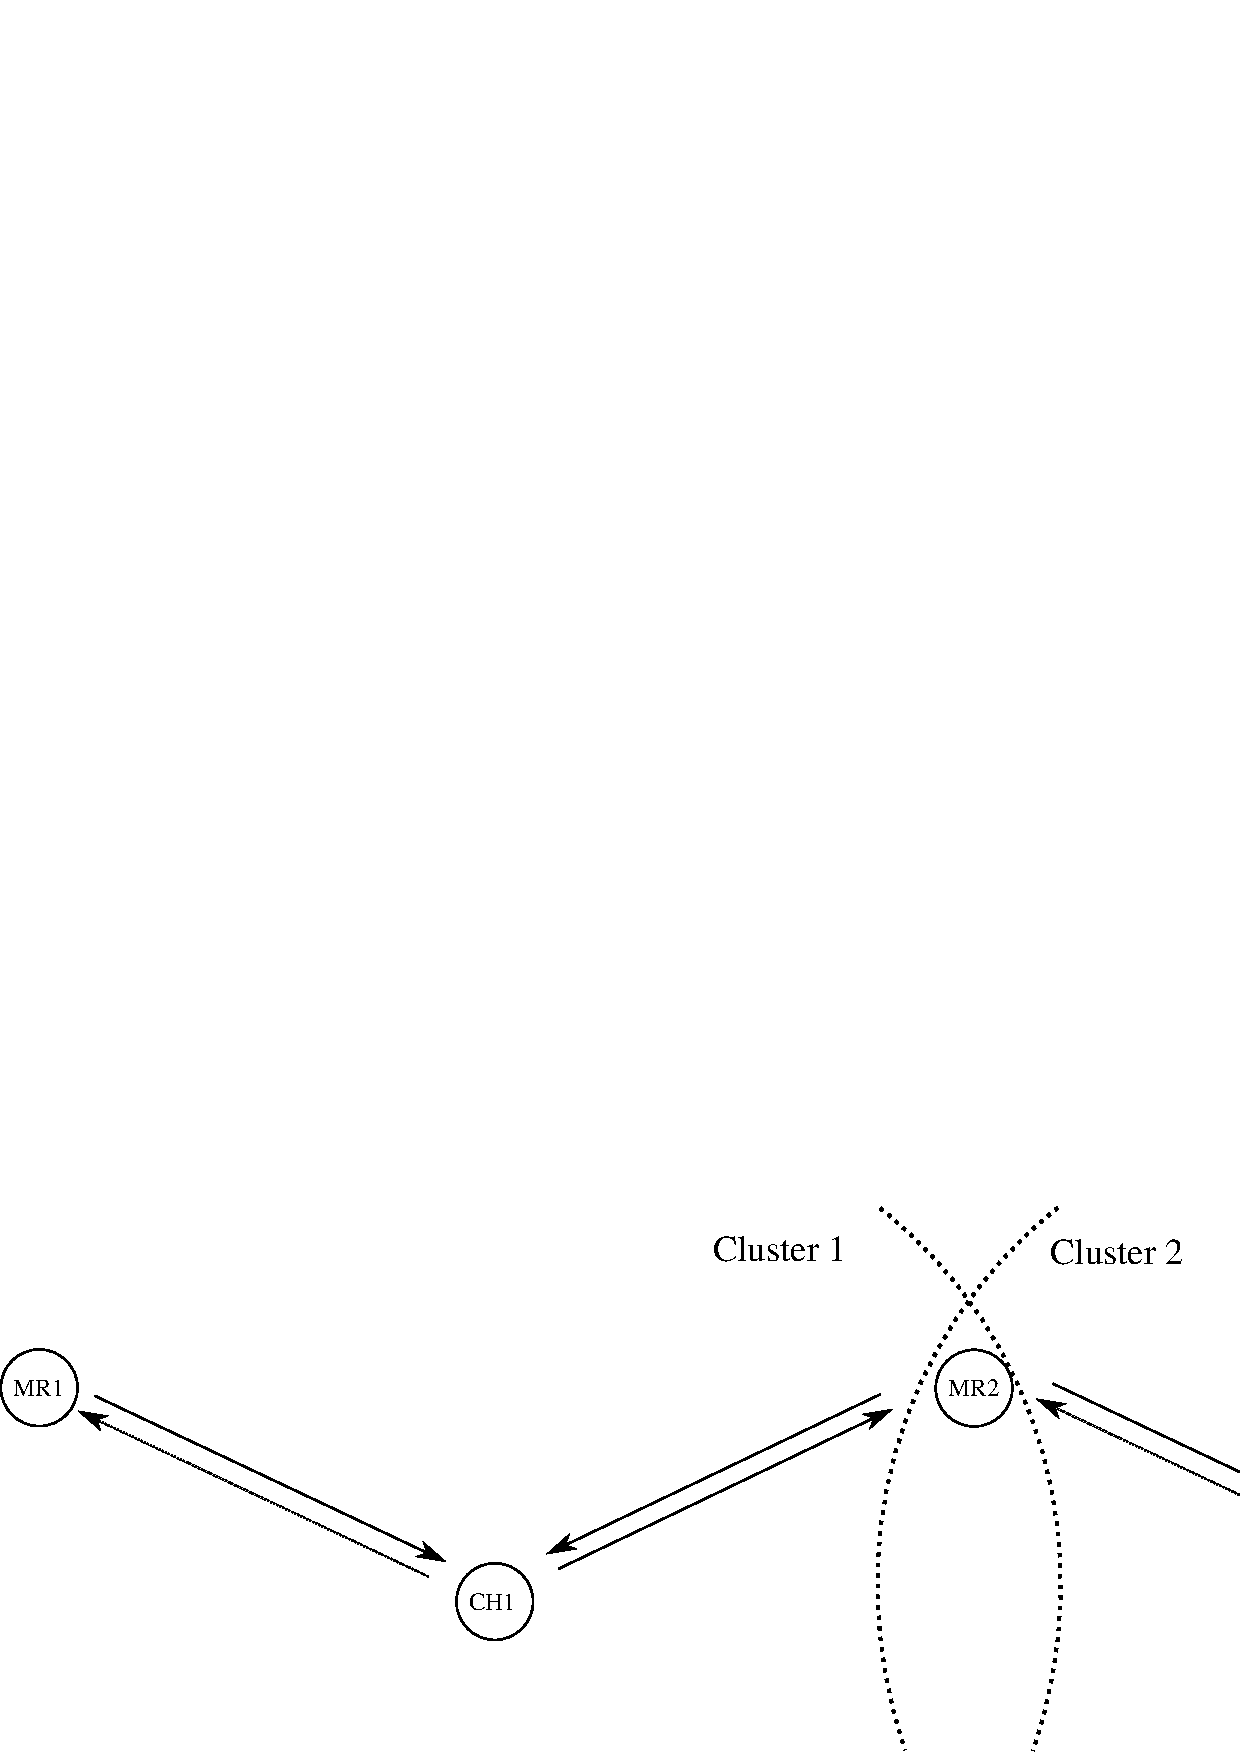
\includegraphics[width=\textwidth]{figures/5nodes}
\caption{The mesh network topology is organized in clusters. Each cluster is controlled by a cluster head (CH). Other nodes in the network are called mesh routers (MR) since they can be used to relay information between CHs.}
\label{fig:mesh_topology}
\end{figure*}

In OpenAirMesh, the network is organized in clusters, where dynamically-allocated cluster-heads (CHs) manage radio resources. CHs are typically the best-connected nodes in a particular geographical area and are synchronized in a distributed fashion by using mesh routers (MRs) on the cluster boundaries. An example of a mesh architecture with 5 nodes is show in Figure \ref{fig:mesh_topology}.

%Isolated Node (IN) and Edge Router (ER). Each node in the topology will assume one of these roles at a given time instant depending on different parameters, namely geographic position, traffic distribution, presence of other access technologies and propagation-related effects which impact connectivity. %It may assume the role of ER in addition to one of the other roles. We now describe in more detail each of these roles.

\subsubsection{Cluster Head}
The primary role of the CH is to manage radio resources in their cluster, much as a base-station would in a cellular network. The cluster is defined as the set of nodes which are characterized by one-hop connectivity with the CH. 
%One-hop connectivity is further defined as the capacity to reliably receive and transmit basic signaling channels with the CH using at least the lowest data-rate communication mode. Reliable communication is defined by a transmission which falls below a maximal error probability threshold. 
CH can only be connected to MR on the same frequency-carrier since they use the same temporal resources as other CH. Thus direct CH $\leftrightarrow$ CH communication is not possible on the same frequency carrier. The downlink (CH $\rightarrow$ MR) signaling channels allow for the CH to schedule transmission of labels (in the form of time and frequency mappings on the radio resource) which each carry different types of traffic throughout the mesh network according to pre-defined quality-of-service (QoS) descriptors. The Uplink (UL) signaling channels (MR $\rightarrow$ CH) are used for relaying bandwidth requirement indicators and channel quality measurements from nodes within the cluster. These feed the scheduling algorithms residing in the CH and allow for proper resource allocation satisfying QoS negotiations carried out using Layer 3 (L3) signaling.  The latter are beyond the scope of the description in this paper.

\subsubsection{Mesh Router}
The primary role of an MR is to interpret the scheduling information from the CH on the downlink (DL) signaling channels in order to route the traffic corresponding to the scheduled labels on the allocated physical resources. MR can be connected to other MR (direct link) in the same cluster. MR can also be connected to more than one cluster at the same time. Since all clusters operate in the same frequency band MR must be able to cancel interference. See Section \ref{sec:ic} for details.

%It is also expected to using the UL signaling channels to relay measurements (both traffic and radio signal) to the CH with which it is connected.
 


\subsection{Layer 2 Protocol Stack}
\label{sec:mac}

The OpenAirMesh Layer 2 protocol stack comprises:
\begin{itemize}
\item  A IP/MPLS networking device (non-access stratum (NAS) driver) responsible for provision of IP/MPLS layer services to Layer 2 and vice-versa
\item  A Radio resource control (RRC) entity responsible for MAC layer signaling for configuration of logical channels and retrieval of measurement information.
\item A Radio Link Control (RLC) entity which is responsible for hybrid automatic repeat request (HARQ) protocols and IP packet segmentation
\item A convergence protocol (PDCP) responsible for IP interface and related functions (header compression, ciphering, etc.)
\item A scheduling and multiplexing unit to control the media access (MAC). 
\end{itemize}
An overview of the layer 2 protocol stack for a CH is shown in Figure \ref{fig:Layer2_stack} and a subset of these entities are described in the following subsections. 

\begin{figure}
 \includegraphics[width=\columnwidth]{figures/layer2_stack}
\caption{OpenAirMesh CH Layer 2 Protocol Stack}
\label{fig:Layer2_stack}
\end{figure}

\subsubsection{Radio Resource Control (RRC)}
The radio resource control entity is responsible for the L2 signaling implementing the radio bearer establishment and maintenance through the control of measurement procedures. Its internal state machine controls the basic procedures for startup, monitoring of synchronization through the measurement system and update of the node's role in the network. RRC is responsible for configuration of all layer 2 entities (and PHY via MAC), both dynamic (during flow establishment) and static (control channels). This functionality is in response to events occurring in the interaction with L3 and based on dynamic measurements of radio quality and traffic intensity. 

% Two types of low-layer measurements are available to RRC.  The first corresponds to measurements of an established radio bearer, which is used to monitor the quality of a link.  The available measurements for CH RRC(L2) are: 
% \begin{enumerate}
% \item	RSSI (dBm) on physical resources corresponding to logical channel.
% \item Average SINR (dB) on physical resources corresponding to logical channel.
% \item Average number of transmission rounds on transport channel associated with logical channel.
% \item Average residual block error rate on transport channel associated with logical channel (after HARQ).
% \item Actual Spectral efficiency of transport channel associated with logical channel.
% \end{enumerate}


\subsubsection{Radio Link Control (RLC)}
The RLC segments IP packets. The segment size is configurable for each QoS class and is signaled by higher layers during route establishment. The sizes are chosen based on the granularity of the underlying MAC/PHY resources (transport blocks).  RLC is responsible for ARQ and indexing of service data units (SDUs) from the user traffic and signaling SDUs from RRC. The SDU inputs from PDCP form the set of radio bearers, and those from RRC the set of signaling radio bearers. It has three modes of functionality: acknowledged (AM), unacknowledged (UM) and transparent (TM). Each logical channel in AM has an associated selective-repeat ARQ process which is managed by RLC which is meant to provide a third level of error recovery with respect to the FEC offered by PHY and HARQ by MAC. The ARQ mechanisms are based on Release 6 3GPP RLC (25.322) specifications. The interface with RRC serves for the configuration of the radio bearer. The interface with MAC is designed such that data for each logical channel is buffered in data queues, whose occupancy can be measured by the MAC scheduling entity.

\subsubsection{MAC Scheduling Entity (MAC)}
The MAC layer scheduling and multiplexing entity is responsible for scheduling control plane and user plane traffic on the physical OFDMA resources. On transmission, the inputs to this entity are connected to data queues originating in the RLC layer which form the set of logical channels. The control plane traffic is represented by the following logical channels:
\begin {itemize}
 \item Broadcast Control Channel (BCCH): This resource is a low bit-rate control channel used by a CH for broadcasting basic information to nodes in the cluster.
\item Common Control Channel (CCCH): This resource is a low bit-rate control channel used both during the attachment or association phase of a new node.
\item Dedicated Control Channel (DCCH): This is a resource used to relay access-layer signaling information (RLC return channels, RF measurement reporting, traffic measurement reporting, power control, etc.) to the corresponding node.
\end{itemize}
The user plane traffic is represented by the following logical channel:
\begin {itemize}
\item Dedicated Traffic Channel (DTCH): This resource is a variable bit-rate traffic channel with negotiated QoS parameters used by the mesh network to transport data traffic corresponding to a particular flow.
\end {itemize}
It is important to note that although dedicated resources are configured at the input of the MAC layer, the physical resources allocated in the scheduling entities (with exception of the CHBCH) are dynamically allocated every CH transmission time interval (TTI) and thus all physical resources are shared. The BCCH is multiplexed in the scheduling entity responsible for generation of the CH-BCH transport channel along with MAC-layer signaling. MAC signaling concerns both allocations of CH-SACH in the current frame and MR-SACH in the next frame (uplink, downlink and direct link map of PHY resources). The CCCH (uplink) is used exclusively during the attachment phase of the MR with a particular cluster and corresponds to the only random-access resources allocated by the CH in the frame. 
\begin{figure}
 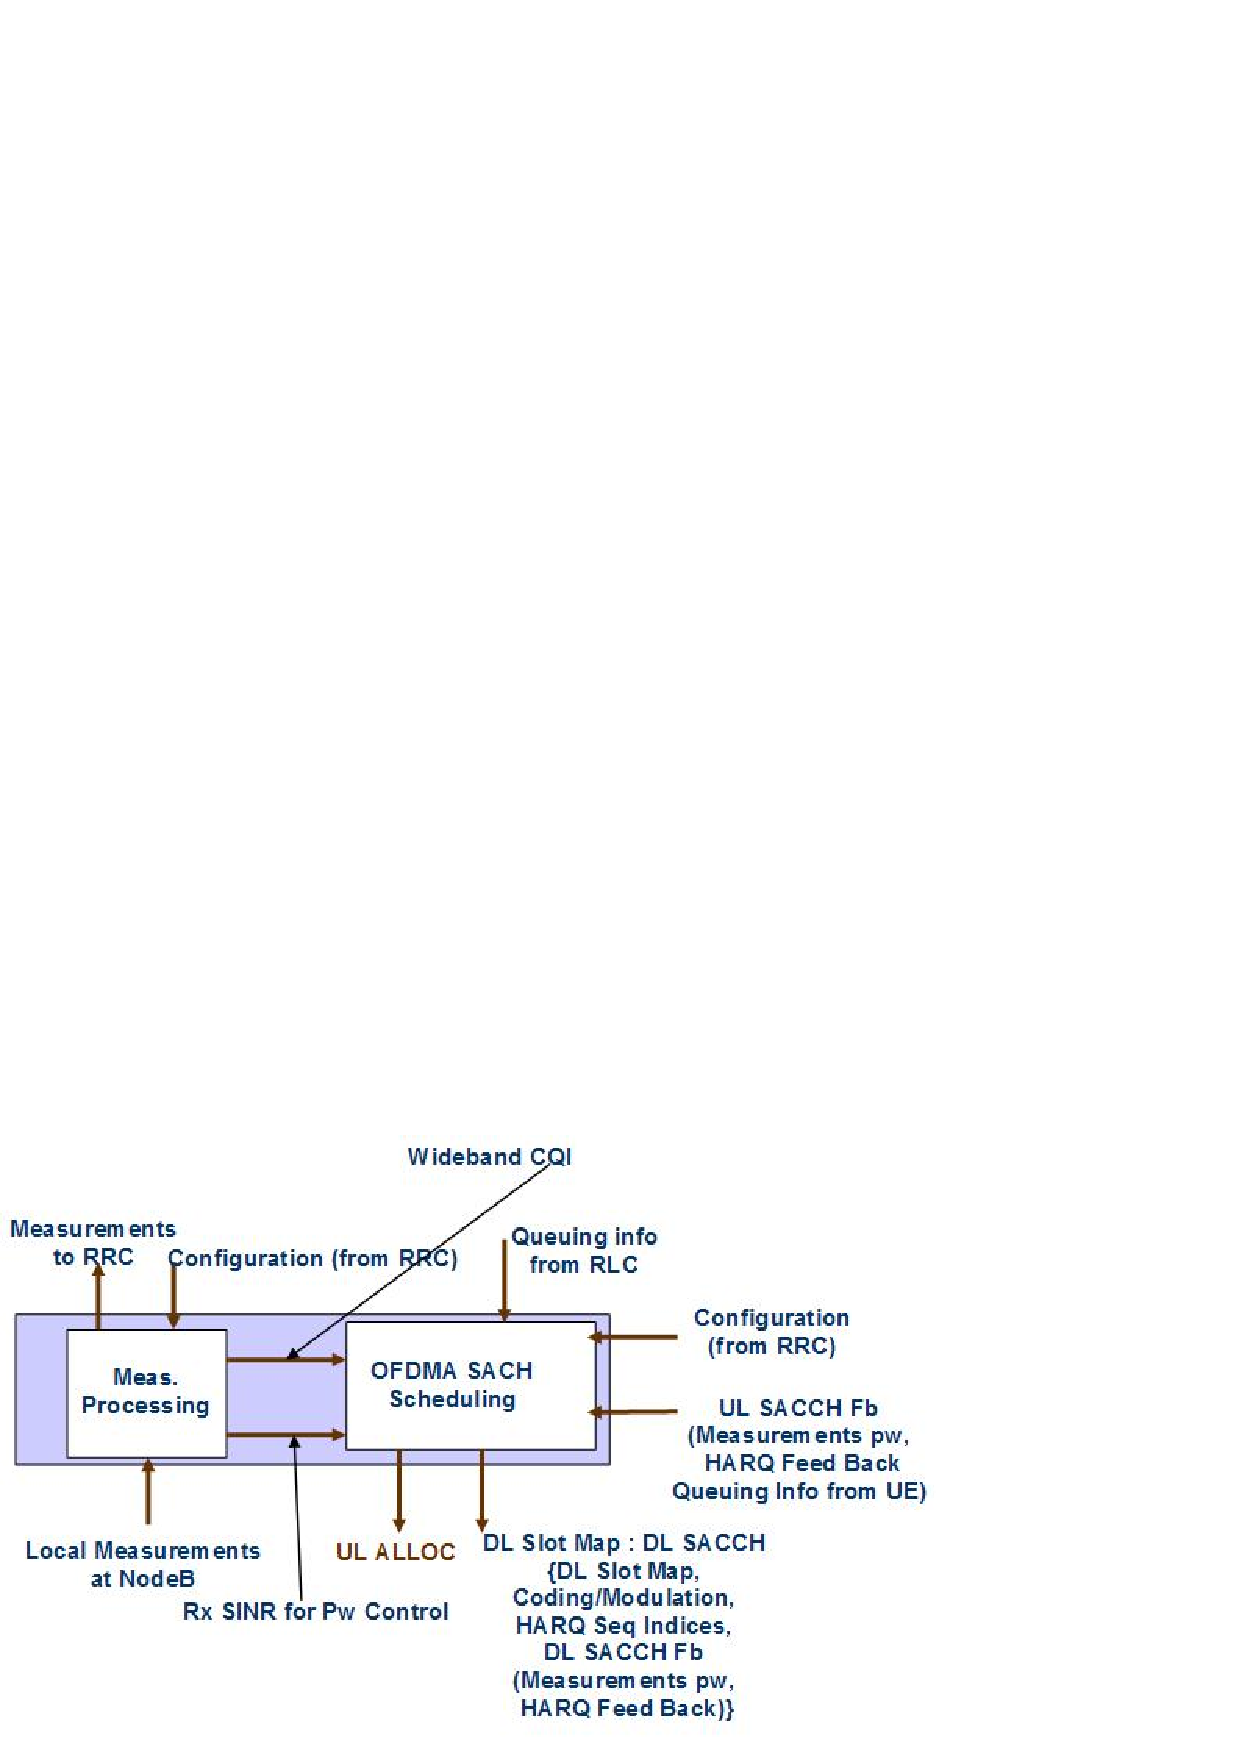
\includegraphics[width=\columnwidth]{figures/sched}
\caption{Overview of the MAC Scheduler}
\label{fig:scheduling}
\end{figure}

The DCCHs are multiplexed along with user-plane traffic DTCHs on the available CH-SACH resources. Based on measurement and feedback information, SACH scheduling (see Figure \ref{fig:scheduling})  aims to respect the negotiated QoS of each logical channel, while maximizing the aggregate spectral efficiency of the data streams. Different wideband scheduling policies taking into account both queuing measures from RLC and channel quality feedback can be accommodated (see for instance \cite{pap:Realp06}).  Channel quality information is signaled between corresponding MAC-layers based quantized wideband channel estimates received from PHY. 

As a general rule, DCCH and CCCH do not use HARQ, since they are signaling channels which use the lowest spectral efficiency modulation. DTCH generally uses HARQ with a maximum number of retransmission rounds determined by higher layer configuration (i.e., the delay class in the QoS requirement). SACH scheduling makes use of up to 16 parallel HARQ Type-2 processes per logical channel in order to maximize throughput and benefit from superior channel conditions.


%The MAC entity is responsible for scheduling control plane and user-plane traffic on the physical OFDMA resources. On transmission, the inputs to this entity are connected to data queues originating in the RLC layer which form the set of logical channels. The control plane traffic is represented by logical channels which form the interface with the RLC. Logical channels contain both user-plane (originating in the IP/MPLS entity via the PDCP entity) and control-plane traffic (originating in the RRC entity). MAC layer specifications are found in Cellular MAC Layer (MAC) Specifications. The MAC is responsible the transport channel interface which exchange data (MAC SDUs) and PHY measurement data for RRC measurement procedures.

\subsection{Physical Layer}
\label{sec:phy}

The physical layer of the platform targets WiMax and UMTS LTE like networks and thus uses multiple-input multiple-output orthogonal frequency division multiple access (MIMO-OFDMA) as modulation and multiple access technique. The actual parameters and mechanisms can be configured prior to deployment of the equipment or potentially over-the-air, although the latter is not yet supported by any of the OpenAir MAC implementations.

The MIMO-OFDMA system provides the means for transmitting several multiple-bitrate streams (multiplexed over sub-carriers and antennas) in parallel. Moreover, PHY signaling strategies are included to provide the means for exploiting channel state feedback at the transmitters in order to allow for advanced PHY allocation of OFDMA resources via the MAC.

This section describes the physical and transport channels, the framing and channel multiplexing, the coding and modulation scheme, as well as the synchronization procedure.

\subsubsection{Physical and Transport Channels}

OpenAirMesh uses a layering architecture which strongly resembles that of an ETSI standard, in the sense that data and control traffic flows use radio bearers, logical, transport and physical channels.  Here we are concerned primarily with the MAC and PHY layer description, and thus the transport channel interface. This encompasses the control and user plane interfaces between the MAC and PHY layers and is composed of the following entities
\begin{itemize}
\item The {\bf CH broadcast channel (CH-BCH)} is a broadcast control channel which houses MAC-layer signaling for CH and MR physical resource scheduling as well as layer 2 radio-resource control (RRC) signaling for topology and QoS management. 
\item The {\bf CH Scheduled-Access Channel (CH-SACH)} is a data channel (for both control and user-plane logical channels) used by CH to communicate with a node in its cluster.  It can be configured as a multicast flow or as a unicast flow with an associated MR-SACH in the reverse direction originating in the corresponding node.
\item The {\bf MR broadcast channel (MR-BCH)} is a broadcast resource used by MR to extend the coverage of a cluster during topological discovery. 
\item The {\bf MR Scheduled-Access Channel (MR-SACH)} is a data channel (for both control and user-plane logical channels) used by MR to communicate with a node in one of the clusters with which the MR is associated.  It can be configured as a multicast flow or as a unicast flow with an associated MR-SACH or CH-SACH in the reverse direction originating the corresponding node.  It uses the physical resources allocated by the CH in the CHBCH and is always bundled with an MR-SACCH. 
\item The {\bf MR Scheduled-Access Control Channel (MR-SACCH)} is a MAC-layer signaling channel associate to a particular MR/CH-SACH used to provide PHY modulation formats for the corresponding MR-SACH in the current TTI as well as feedback information for the HARQ processes and channel quality indicators for the corresponding pair MR-SACH/CH-SACH in the reverse direction. 
\item The {\bf Random-Access Channel (RACH)} is a signaling channel used by a MR during the association phase with the CH. 
\end{itemize}

Each of the transport channels is mapped to a corresponding physical channel of the same name. In addition, two other physical channels used for parameter estimation are also available: 
\begin{itemize}
\item The {\bf Physical CH Synchronization Channel (CHSCH)} is a pilot resource reserved to a CH which is responsible for delivering synchronization information to nodes in the cluster. This channel is used by nodes to acquire timing information regarding the beginning of the TTI and to perform initial frequency offset adjustments with respect to the carrier frequency of the CH. The channel is also used by adjacent CHs to synchronize the network, in order to facilitate inter-cluster communication under quality-of-service guarantees. 
\item The {\bf Physical Synchronization Channel (SCH)} is a pilot resource used by a node to allow the CH to estimate the channel of an MR/UE.
\end{itemize}

\subsubsection{Framing and Channel Multiplexing}

\begin{figure}
 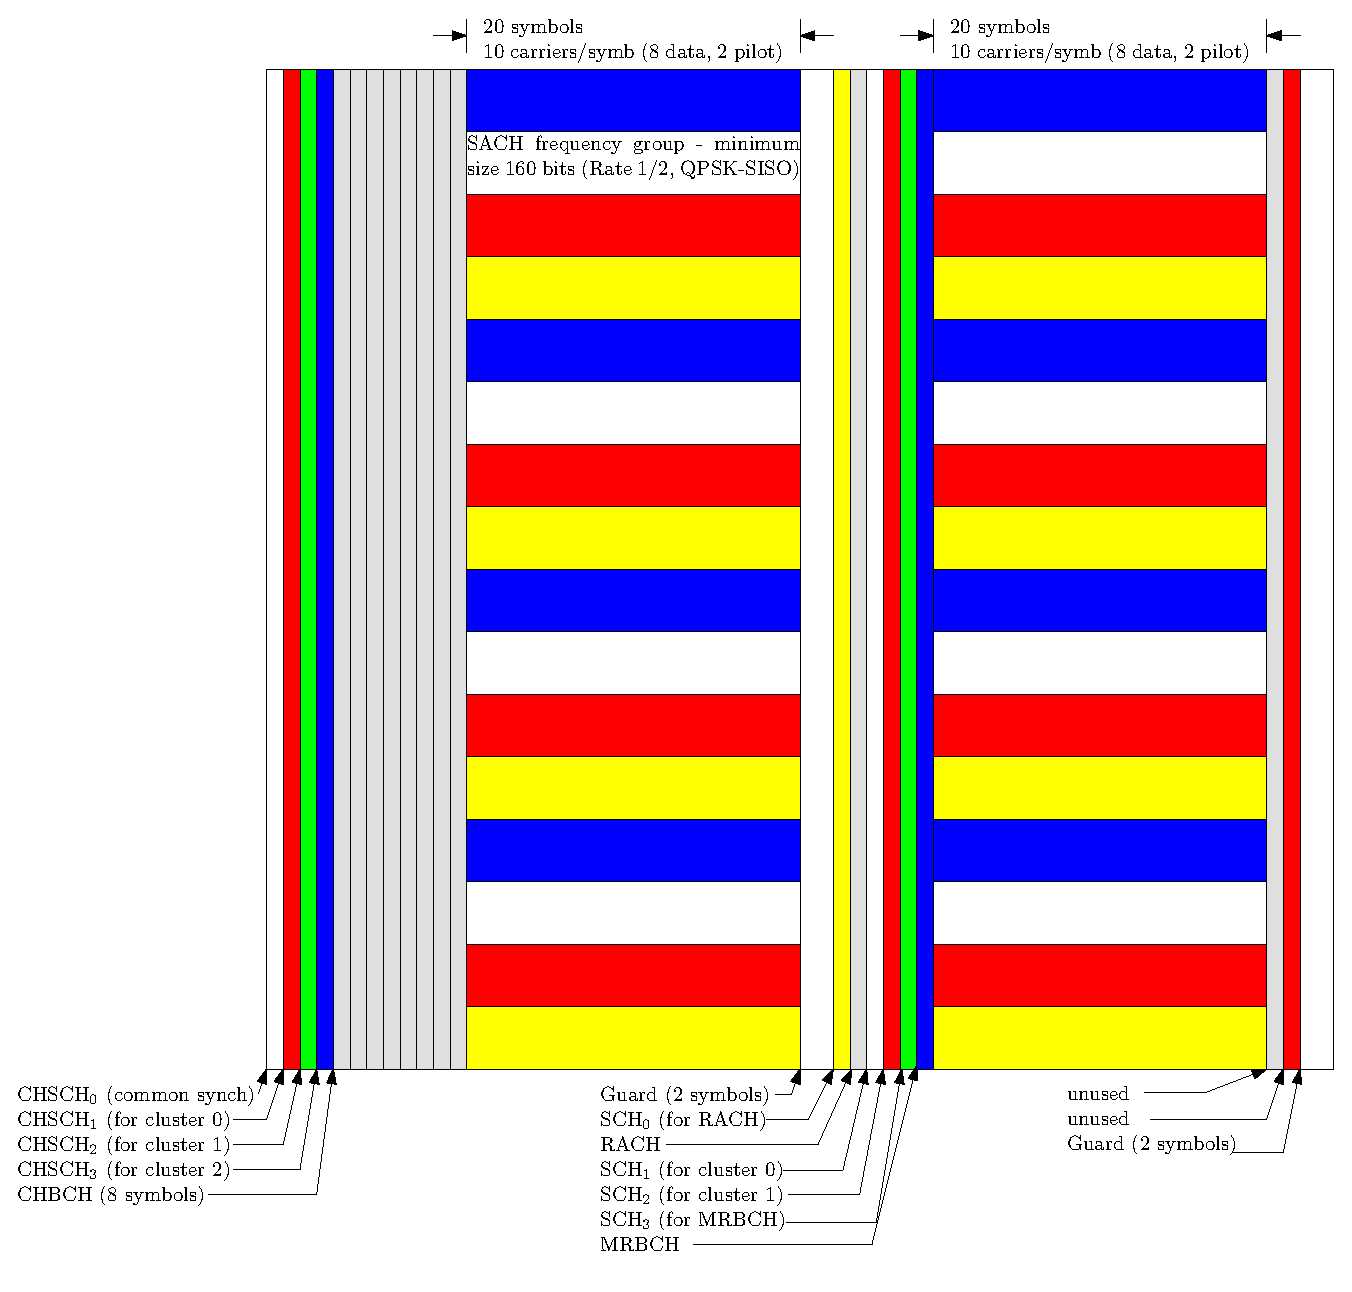
\includegraphics[width=\columnwidth]{figures/mesh_frame}
\caption{Mesh frame structure}
\label{fig:frame_structure}
\end{figure}

\begin{table}
\centering
\begin{tabular}{|c|c|}
  \hline
Sampling rate & 7.68 Msamp/s \\
Symbol (DFT/IDFT) size & 256 samples \\
Prefix length & 64 samples (8.33$\mu$s) \\
Useful carriers & 160 \\
Number of subbands (chunks) & 16 \\
Data carriers per subband & 8 \\
Pilots per subband & 2 \\\hline
\end{tabular}
\caption{Nominal OFDMA Parameters in OpenAirMesh \label{tab:framing}}
\vspace{-0.4cm}
\end{table}

The physical resources are organized in frames of OFDM symbols. OpenAirMesh framing is completely configurable, but the nominal OFDMA configuration is shown in Table \ref{tab:framing}. One frame consists of 64 OFDM symbols and is  divided in a CH transmission time interval (TTI) and a MR TTI (see Figure \ref{fig:frame_structure}). The first four symbols of the CH TTI are reserved for pilot symbols. Each CH transmits one common pilot symbol (CHSCH$_0$) at position 0 and one dedicated pilot symbol (CHSCH$_i$) at position $i \in \{1,2,3\}$. This way we can ensure orthogonality between the pilots of different CH received at one MR. The pilot symbols are followed by the broadcast channel (CH-BCH).  The rest of the CH TTI frame is reserved for the multiplexed scheduled access channels (CH-SACH).


The MR TTI contains the random access channel (MR-RACH) with an associated pilot symbol (SCH$_0$). The next two symbols are reserved for pilots. Each MR transmits a pilot symbol SCH$_i$, $i \in \{1,2\}$ corresponding to the cluster it belongs to. This way we can ensure orthogonality between the pilots of different CHs. 
%[why do we need this? on the uplink the pilots do not interfeer, do they?]. 
The pilot symbols are followed by the uplink broadcast channel (MR-BCH) with an associated pilot symbol (MRSCH). The rest of the uplink frame contains the multiplexed scheduled access channels (MR-SACH). The end of the CH and MR TTIs are protected by a guard interval of two symbols. All pilots are designed for MIMO and/or Multiuser channel estimation at the corresponding end. 



\subsubsection{Coding and Modulation}
\label{sec:coding}

\begin{figure*}
\centering
 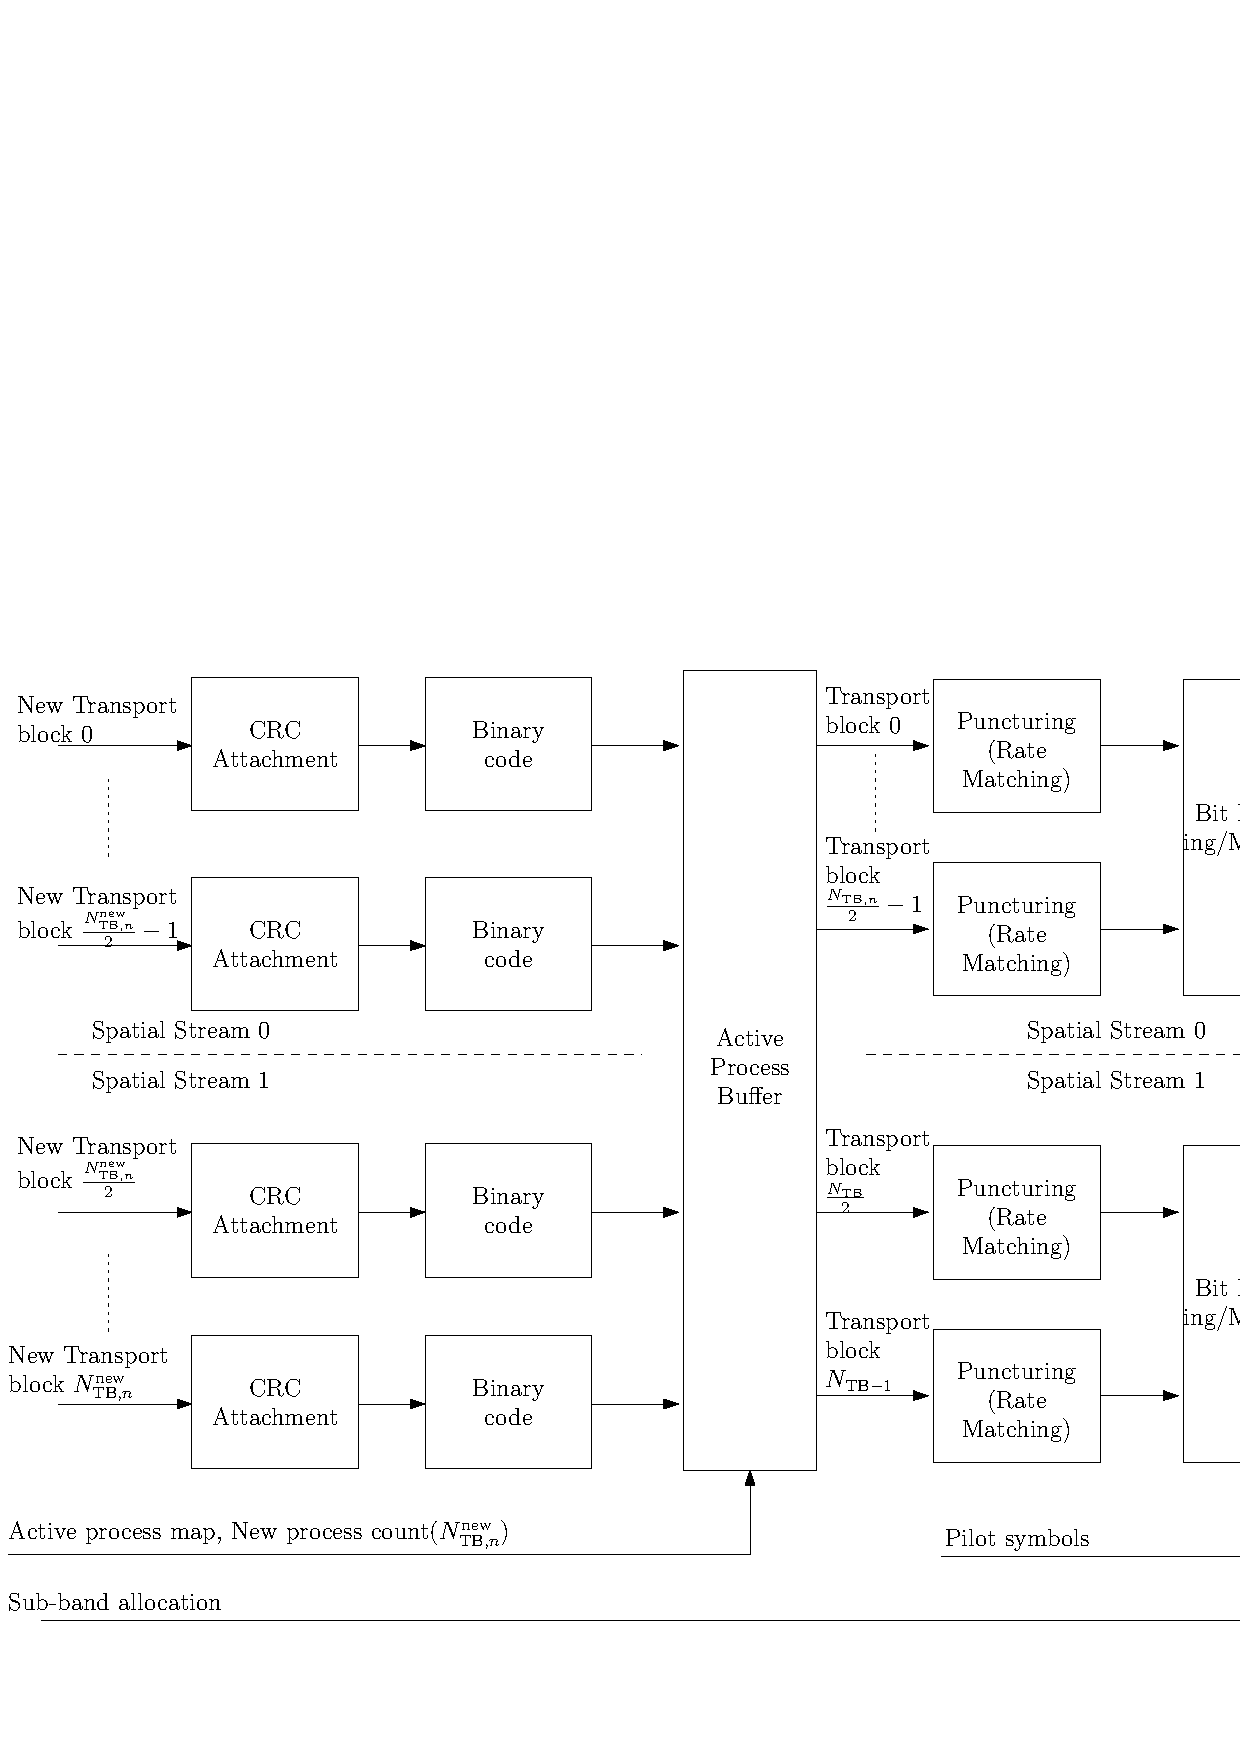
\includegraphics[scale=.5]{figures/openair_coding}
\caption{OpenAirMesh Coded Modulation and HARQ}
\label{fig:coding}
\end{figure*}

OpenAirMesh makes use of punctured binary codes (64-state rate 1/2 convolutional or 8-state rate 1/3 3GPP/LTE Turbo code). Puncturing can use either 3GPP rate matching or random puncturing in order to fine tune the coding rate to adapt to configurable transport block sizes delivered to PHY by the MAC.  The overall coding sub-system is shown in Figure \ref{fig:coding}. New transport blocks arriving from the MAC layer (based on multi-user scheduling) are coded using a CRC extension and the chosen binary code.  These are then fed to the active transport block buffer along with those that are to be retransmitted.  Each transmitted block is punctured and then passed to a bit-interleaver and modulation mapper (BICM).  OpenAirMesh supports QPSK, 16-QAM and 64-QAM modulation although currently only QPSK is used.  The transmitted transport blocks can be split into to two spatial streams in the case of point-to-point MIMO transmission.

The modulated symbols are then multiplied by an adjustable amplitude and passed to the space-time-frequency (STF) parser. The STF parser multiplexes the pilot symbols and the data symbols into OFDM symbols, taking into account the sub-band allocation from the scheduler. In the case of one available spatial stream the STF parser also performs fast antenna cycling, i.e., every subcarrier is transmitted from a different antenna. This way each stream sees all the degrees of freedom of the channel. In the case of two spatial streams the STF parser guarantees that both streams use different antennas in the same time/frequency dimension.  This is a form of superposition coding since the two streams are combined additively in the air through the use of multiple transmit antennas. 

This design allows to use the same transmitter and receiver structure both for point-to-point MIMO as well as distributed MIMO transmission. In the latter case one spatial stream is used at each source and the second stream originates in another part of the network, either in the same cluster or an adjacent cluster.  A particular user can decode both streams or simply select the one it requires. In Section \ref{sec:ic} we derive a low-complexity successive interference cancellation (SIC) receiver for this design. 


\subsubsection{Network Synchronization Procedure}
\label{sec:sync}

The OpenAirMesh network supports full time synchronization. Synchronization is achieved by declaring one CH to be the primary CH, which is the reference clock in the system. Every MR within this cluster synchronizes to the CH using the CHSCH. The MRs then collaborate as a distributed array by sending out a synchronization signal themselves (the MRSCH) to allow a secondary CH (not within the broadcast domain of the primary CH) to synchronize to the network. As soon as a secondary CH is synchronized to the network, it also sends out a CHSCH, allowing further MRs to synchronize, and so on.  This type of distributed synchronization can be interpreted as a form of {\em firefly synchronization} \cite{tyrell06fireflies,hu06scalability}. However, it is not completely distributed because it requires the presence of a reference clock in the system. 

% We now sum up the initial synchronization procedure during network establishment. When a node is turned on, it first looks for a CHSCH$_i$ $i=1,2,3$ and tries to decode the corresponding CHBCH. If successful it declares itself synchronized to CHSCH and becomes a MR. Otherwise it looks for a MRSCH and tries to decode MRBCH. If successful, it declares itself synchronized to MRSCH and becomes a secondary CH. Otherwise it becomes a primary CH. 

% \subsubsection{Channel Estimation}
% 
% Explain the pilot structure and how we obtain channel estimates from both clusters. 

\section{Dual-stream Interference Cancellation Receiver Architecture}
\label{sec:ic}

The key ingredient for allowing spatial reuse one in wireless networks is interference mitigation. In the mesh architecture described in the previous section, MRs that are between two CHs must be able to communicate concurrently with both CHs (one stream for each CH on transmit and receive) on the same  time-frequency resources since the scheduling between clusters is not coordinated. In this section we describe two different dual-stream multi-antenna receiver structures that can be used for this purpose, namely an MMSE receiver (see Subsection \ref{sec:MMSE}) and an approximate ML receiver (see Subsection \ref{sec:ML}) \cite{ghaffar08b,ghaffar08c}. The derivations are based on the signal model presented in Subsection \ref{sec:signal_model}. Both receivers were first implemented in Matlab and later on the OpenAirInterface platform. In the next Section we then show performance comparisons of both implementations in a synthetic simulation environment as well as from a real-time over-the-air lab test.

\subsection{Signal Model}
\label{sec:signal_model}

Consider the scenario depicted in Fig.\ \ref{fig:mesh_topology} with two clusterheads but only one MR (MR2). We assume that each CH has $n_{t}$ antennas and MR2 has $n_{r}$ antennas. Let $\textbf{x}^{(j)}_{m,q}$ denote $n_{t} \times 1$ vector of the transmit symbols for subcarrier $q$ of OFDM symbol $m$ of CH $j,~j=1,2$. We assume that the transmit symbols are taken from a signal set $\chi_{j}\subseteq\mathbb{C}$ of size $\left|\chi_{j}\right|=M_{j}$ with a Gray labeling map $\mu_{j}:\left\{0,1\right\}^{\log\left|M_{j}\right|}\rightarrow \chi_{j}$ while $j\in\left[1,2\right]$.

Cascading the IFFT at the MR and the FFT at the CHs with CP extension, the received signal at MR2 at $q$-th frequency tone and the $m$-th OFDM symbol can be expressed as:
\begin{equation}
\label{eqn:sys_model}
\Vec{y}_{m,q} = \Mat{H}^{(1)}_q \Vec{x}^{(1)}_{m,q} + \Mat{H}^{(2)}_q \Vec{x}^{(2)}_{m,q} + \Vec{z}_{m,q}
\end{equation} 
where $\Mat{H}^{(1)}_q$ and $\Mat{H}^{(2)}_q$ denote the $n_{r} \times n_{t}$ MIMO channel between CH1 and MR2 and between CH2 and MR2. The channel is assumed to be frequency selective (i.e., it varies with subcarrier index $q$) and block fading (i.e., constant over the OFDM symbols of a frame). $\textbf{z}_{m,q}\in\mathbb{C}^{n_{r}}$ is the vector of circularly symmetric complex white Gaussian noise of variance $\sigma^2$.

Since each clusterhead transmits only one spatial stream and antenna cycling is used, only one element of  $\textbf{x}^{(j)}_{m,q},~j=1,2$ is non-zero for every $m$ and $q$. We identify this non-zero element with  $x^{(j)}_{m,q},~j=1,2$ and can rewrite \eqref{eqn:sys_model} equivalently as 
\begin{equation}\label{eq:cellularfreq}
\textbf{y}_{m,q}\!=\!\textbf{h}^{(1)}_{q}x^{(1)}_{q,m}+\textbf{h}^{(2)}_{q}x^{(2)}_{m,q}+\textbf{z}_{m,q},
\end{equation}
where $\textbf{h}^{(1)}_{q}$ and $\textbf{h}^{(2)}_{q}$ are the equivalent channel vectors for the non-zero elements.  
%	
% where $K$ is the total number of frequency tones. $q\in\left[0,1,\cdots,n_{t}\right]$ shows antenna cycling at CH with the channel vector taking $n_{t}$ different values. We assume that the subcarriers are narrowband and model each subcarrier as a frequency flat fading channel so $\textbf{h}_{1,k,q}\in\mathbb{C}^{n_{r}}$ is the vector characterizing flat fading channel response from CH-1 to $n_{r}$ receive antennas at MR at the $k$-th subcarrier. This vector has complex-valued multivariate Gaussian distribution with $E\left[\textbf{h}_{1,k,q}\right]=\textbf{0}$ and $E\left[\textbf{h}_{1,q}\textbf{h}_{1,q}^{\dag}\right]=\textbf{I}$ i.e. each channel between the CH and the $n_{r}$ receive antennas of MR is independent while the channels at different subcarriers are also assumed to be independent. Each subcarrier corresponds to a symbol from a constellation map $\chi_{j}$ for the $j$-th stream. $\textbf{y}_{k}$, 
%
The complex symbols $x^{(1)}_{m,q},x^{(2)}_{m,q}$ of the $2$ streams are assumed to be independent and of variances $\sigma^{2}_{1}$ and $\sigma^{2}_{2}$ respectively. Assuming that the first stream is the desired stream, the signal to noise ratio (SNR) is given by ${\sigma^{2}_{1}}/{\sigma^2}$ and the signal to interference ratio (SIR) by ${\sigma^{2}_{1}}/{\sigma^{2}_{2}}$.


For notational convenience, we can drop the frequency and OFDM symbol indexes and rewrite the system model as
\begin{align}\label{eq:cellularfreq1}
\textbf{y}&=\textbf{h}_{1}x_{1}+\textbf{h}_{2}x_{2}+\textbf{z}\nonumber\\
\textbf{y}&=\textbf{H}\textbf{x}+\textbf{z}\nonumber
\end{align}
where $\textbf{H}=\left[\textbf{h}_{1}\;\textbf{h}_{2}\right]$ and $\textbf{x}=\left[x_{1},x_{2}\right]^{T}$.



\subsection{MMSE Receiver}
\label{sec:MMSE}
Linear spatial filters as minimum mean square error (MMSE) and zero forcing (ZF) filters are the focus of attention to minimize the level of interference in the former case while nulling out the interference in the latter case. Linear MMSE filters because of comparatively better performance than ZF are being considered as likely candidates for future wireless systems \cite{Ericsson}. The sub-optimality of MMSE for non Gaussian alphabets in low dimensional systems (less number of interferers) is well known \cite{Poor} and moreover MMSE detection being based on interference attenuation is void of exploiting the interference structure in mitigating its effect. 
%where $\chi_{1,c_{k^{'}}}^{i}$ denotes the subset of the signal set $x_{1}\in\chi_{1}$ whose labels have the value $c_{k^{'}}\in\left\{0,1\right\}$ in the position $i$. This metric has computational complexity $\mathcal{O}\left(\left|\chi_{1}\right|\right)$.

Detection based on MMSE equalization \cite{Medvedev} involves linear MMSE pre-processing i.e. applying a spatial filter \textbf{M} to the received signal vector $\textbf{y}$ i.e. $\tilde{\textbf{x}}=\textbf{My}$ where $\tilde{\textbf{x}}$ is the biased estimate of $\textbf{x}$. Frequency domain MMSE filter \textbf{M} is given as
\begin{equation}\label{eq:MSSEeqn1}
\textbf{M}=\left(N_{0}\textbf{P}^{-1}+\textbf{H}^{H}\textbf{H}\right)^{-1}\textbf{H}^{H}\nonumber
\end{equation}
where $\textbf{P}$ is the diagonal power distribution matrix with the diagonal as $\left[\sigma^{2}_{1}, \sigma^{2}_{2}\right]$. It is followed by an unbiasing operation i.e. $\hat{\textbf{x}}=\Gamma^{-1}\tilde{\textbf{x}}$ where $\Gamma=\mbox{diag}\left(\textbf{M}\textbf{H}\right)$.
Post detection interference is assumed to be Gaussian which on one hand reduces the computational complexity but on the other adds to the sub-optimality of MMSE detection. MMSE pre-processing decouples the spatial streams and the bit metric for the $i$-th bit for bit value $b$ of the symbol $x_{k}$ on $k$-th stream is given as
\begin{equation}\label{eq:MSSEeqn3}
\lambda^{i}_{k}\left(\textbf{y},b\right)\approx \max_{x_{k}\in\chi^{i}_{k,b}}\left[-\frac{\gamma_{k}^{2}}{N_{0}}\left|\hat{x_{k}}-x_{k}\!\right|^{2}\right]
\end{equation}
for $k=1,2$ where $\gamma_{k}$ is the $i$-th diagonal element of $\Gamma$. $\chi_{k,b}^{i}$ denotes the subset of the signal set $x_{k}\in\chi_{k}$ whose labels have the value $b\in\left\{0,1\right\}$ in the position $i$. Based on these bit metrics, bit log likelihood ratios (LLRs) are calculated which after de-interleaving are passed to the channel decoder.


\paragraph*{Implementation}

The core of the MMSE receiver is the matrix inversion that is needed to calculate the filter 
$$\Mat{M} = {\underbrace{(N_0 \Mat{P}^{-1} + \Mat{H}^H\Mat{H})}_{=:\Mat{A}}}^{-1} \Mat{H}^H.$$
$\Mat{M}$ needs to be calculated for every subcarrier and every frame, but we drop the indices for notational convenience. 
 
Since we are limited to a $2 \times 2$ MIMO system, the matrix inversion can be calculated directly using Cramer's rule $A^{-1} = \frac{1}{\operatorname{det}(\Mat{A})} \operatorname{adj}(\Mat{A})$, where $\operatorname{adj}(\Mat{A})$ denotes the adjoint of the matrix $\Mat{A}$.   
Care has to be taken to properly scale the intermediate results in a fixed point implementation. The entries of the channel matrices $\Mat{H}$ are stored in signed 16bit-wide variables, but their resolution is limited to 12 bit due to the A/D convertors. Since the calculation of the determinant $\operatorname{det}(\Mat{A})$ involves terms up to the fourth power, the dynamic range of the determinant can reach up to 48 bit. In order to handle this high dynamic range we first use a 64bit-wide variable to calculate $\operatorname{det}(\Mat{A})$ thus not loosing any accuracy. This intermediate result is then shifted such that $\max{\operatorname{det}(\Mat{A})}$ uses 16 bits. In order to calculate the inverse of $\operatorname{det}(\Mat{A})$, we interpret all numbers as fractional Q15 numbers and use standard fixed-point arithmetic. Intermediate results are stored in double precision. The inverse is scaled back by the mean (over all subcarriers) of $\operatorname{det}(\Mat{A})$ and saturating to 16bit. 

Finally, the MMSE filter matrix is calculated according to $\Mat{M} = \frac{1}{\operatorname{det}(\Mat{A})} \operatorname{adj}(\Mat{A}) \Mat{H}^H$, scaling the intermediate results always to 16 bits. 

The high dynamic range of the determinant can cause severe problems. Especially in a frequency selective channel the inverse may saturate on some carriers and can be zero on some other frequencies. This will become more evident in the result section.  



\subsection{Low Complexity max log MAP Detector}
\label{sec:ML}
This detector is a low complexity version of max log MAP detector and is based on the matched filter outputs \cite{ghaffar09a}. Its low complexity is based on the reduction of one complex dimension. This detector instead of attenuating the interference exploits its structure in mitigating the effect of interference. Without loss of generality, let's consider first stream being the desired stream. The max log MAP bit metric for bit $b$ of the desired stream $x_{1}$ is given as \cite{caire}
\begin{align}
\lambda^{i}_{1}\left(\textbf{y},b\right)\!&\approx\! \min_{x_{1}\in\chi^{i}_{1,b},x_{2}\in\chi_{2}}\!\left\|\textbf{y}\!-\!\textbf{h}_{1}x_{1}\!-\textbf{h}_{2}x_{2}\right\|^{2}\nonumber\\
&=\!\min_{x_{1}\in\chi^{i}_{1,b},x_{2}\in\chi_{2}}\left\{\left\|\textbf{y}\right\|^{2}\!+\!\left\|\textbf{h}_{1}x_{1}\right\|^{2}\!-\left(2y_{1}x_{1}^{*}\right)_{R}\right.\nonumber\\
&\quad\left.+\left(2p_{12}x_{1}^{*}x_{2}\right)_{R}-\left(2y_{2}x_{2}^{*}\right)_{R}+\left\|\textbf{h}_{2}x_{2}\right\|^{2}\right\}\label{eq:bitLLR}
\end{align}
where $y_{1}=\textbf{h}_{1}^{H}\textbf{y}$ be the matched filter output for the first stream and $p_{12}=\textbf{h}_{1}^{H}\textbf{h}_{2}$ be the cross correlation between the first and the second channel. Note that subscripts $\left(.\right)_{R}$ indicates the real part. Writing terms in their real and imaginary parts, we have
\begin{align}
&\lambda^{i}_{1}\left(\textbf{y},b\right)\approx\min_{x_{1}\in\chi^{i}_{1,b},x_{2}\in\chi_{2}}\left\{\left\|\textbf{h}_{1}x_{1}\right\|^{2}-\left(2y_{1}x_{1}^{*}\right)_{R}\right.\nonumber\\
&\!+\!\left(2\left(p_{12,R}x_{1,R}\!+\!p_{12,I}x_{1,I}\!\right)\!-\!2 y_{2,R}\!\right)x_{2,R}\!+\!\left\|\textbf{h}_{2}\right\|^{2}x_{2,R}^{2}\nonumber\\
&\left.\!+\!\left(2\left(p_{12,R}x_{1,I}\!-\!p_{12,I}x_{1,R}\!\right)\!-\!2 y_{2,I}\!\right)x_{2,I}\!+\!\left\|\textbf{h}_{2}\right\|^{2}x_{2,I}^{2}\right\}\label{eq:MAP1e}
\end{align}
where $\left(.\right)_{I}$ indicates imaginary part. For $x_{2}$ belonging to the equal energy alphabets, the values of $x_{2,R}$ and $x_{2,I}$ which minimize (\ref{eq:MAP1e}) need to be in the opposite directions of $2\left(p_{12,R}x_{1,R}\!+\!p_{12,I}x_{1,I}\right)\!-\!2 y_{2,R}$ and $2\left(p_{12,R}x_{1,I}\!-\!p_{12,I}x_{1,R}\!\right)\!-\!2 y_{2,I}$ respectively thereby evading search on alphabets of $x_{2}$ and reducing one complex dimension of the system. The bit metric is therefore written as
\begin{align}
&\lambda^{i}_{1}\left(\textbf{y},b\right)\approx\min_{x_{1}\in\chi^{i}_{1,b},x_{2}\in\chi_{2}}\left\{\left\|\textbf{h}_{1}x_{1}\right\|^{2}-\left(2y_{1}x_{1}^{*}\right)_{R}\right.\nonumber\\
&\!-\!\left|\left(2\left(p_{12,R}x_{1,R}\!+\!p_{12,I}x_{1,I}\!\right)\!-\!2 y_{2,R}\!\right)\right|\left|x_{2,R}\right|\nonumber\\
&\left.\!-\!\left|\left(2\left(p_{12,R}x_{1,I}\!-\!p_{12,I}x_{1,R}\!\right)\!-\!2 y_{2,I}\!\right)\right|\left|x_{2,I}\right|\right\}\label{eq:MAP3e}
\end{align}

For non equal energy alphabets, it is the minimization problem of a quadratic function again trimming one complex dimension of the system. In that case, the real and imaginary parts of $x_{2}$ which minimizes (\ref{eq:bitLLR}) are given as
\begin{align}
&x_{2,R}\rightarrow-\frac{\left(p_{12,R}x_{1,R}+p_{12,I}x_{1,I}\right)- y_{2,R}}{\left\|\textbf{h}_{2}\right\|^{2}}\nonumber\\
&x_{2,I}\rightarrow-\frac{\left(p_{12,R}x_{1,I}\!-\!p_{12,I}x_{1,R}\!\right)\!-\! y_{2,I}}{\left\|\textbf{h}_{2}\right\|^{2}}
\end{align}
where $\rightarrow$ indicates the quantization process in which amongst the finite available points, the point closest to the calculated continuous value is selected.

%\paragraph*{Implementation}

The advantage of the reduced complexity max-log MAP detector is that it can be implemented without any division and therefore it is numerically more stable than the MMSE receiver. 

\subsection{Integration into OpenAirMesh}

The interference cancellation receiver described above enables the implementation of a single frequency mesh network. Since each CH schedules the time-frequency resources in its cluster independently (both on the uplink and the downlink) MRs that are in the broadcast domain of two different CHs must also be able to communicate with two CHs concurrently on the uplink and the downlink. In the downlink, the IC receiver is used to decode the signals of both CHs successively by treating the other stream as interference. This also enables the MR to synchronize the two CHs. On the uplink the MR transmit two independent data streams as described in \ref{sec:coding} and the CHs decode only the stream dedicated for them, treating the other one as interference. 

\section{Experiments and Applications}
\label{sec:exp}

In this section we investigate the performance of the two dual-stream receiver structures described in the previous section. Firstly, in Subsection \ref{sec:sim}, we perform computer simulations of the two receiver structures using a simple synthetic channel model. Secondly, in Subsection \ref{sec:lab} we present performance results from the real-time implementation on the OpenAirInterface platform. Last but not least, in Subsection \label{sec:trials}
we present field trial experiments that were conducted within the CHORIST project close to Barcelona, Spain in February 2009. 

All performance comparisons (both for simulation and lab tests) were done using the broadcast channel (BCH) of the primary clusterhead (CH1) with interference from the BCH from the secondary clusterhead (CH2). The BCH uses QPSK modulation and rate 1/2 convolutional code. The block length is 1056bits, which corresponds to 8 OFDM symbols with 132 data subcarriers each. We use 2 antennas on all nodes.

\subsection{Computer Simulations}
\label{sec:sim}

\subsubsection{Channel Model}



For the simulations the $2 \times 2$ MIMO channel matrices $\Mat{H}_q^{(1)}$ and $\Mat{H}_q^{(2)}$ are modeled as spatially white and independent. The channel is assumed to be constant during a block and varies independently between blocks. We use both a frequency flat fading model as well as a frequency selective model. In the frequency flat case the channel matrices stay constant over all subcarriers $q$ with channel coefficients drawn  from a Rayleigh distribution with unit variance. In the frequency selective case we model the channel as a tapped delay line with 8 sample-spaced taps with an exponential power delay profile. Each tap undergoes Rayleigh fading. 


% Each link of the MIMO channels $\Mat{H}^{(l)}, l=1,2$ with channel coefficients $h_{i,j}^{(l)}$ is drawn from a Rayleigh distribution, i.e., $h_{i,j}^{(l)} \in \mathcal{CN}(0,1)$. Channel coefficients of different links as well as of different blocks are independent. 

% Note that the assumptions on the channel model are quite strong and hardly ever fulfilled in real channels. However, it allows to check and compare different algorithms and different implementations.

%The first tap additionally includes a LOS component, whose strength is controlled by the Ricean K-factor $K$. The different elements of the MIMO matrices of one cluster fade independently. The LOS components of two different clusters are correlated by the angle $\alpha$. That means if $\mathbf{H}_{\textrm{LOS},1}$ is the channel matrix of the LOS component of CH 1, the corresponding channel matrix of CH 2 is given by....     

\subsubsection{Simulation Results}

The simulation model described above as well as the two receiver structures described in Section \ref{sec:ic} were implemented in Matlab as well as in fixed-point C. The C simulator however includes the FFT and CP insertion at the transmitter and the corresponding IFFT and CP removal at the receiver. The channel is thus simulated in the time domain rather than in the frequency domain. Also the C implementation does a full channel estimation while the Matlab implementation assumes perfect channel knowledge. We perform Monte Carlo simulations with both implementations and compare the frame error rates of the first stream w.r.t.\ the interference from the second stream. 

Figure \ref{fig:sim_results_MMSE} shows the performance comparison of the two implementations of the MMSE receiver for different SNR levels.  It can be seen that the fixed point C implementation looses approximately 5dB compared floating point implementation in Matlab. The loss is due to the loss of accuracy of the fixed point implementation and the channel estimation errors. 

Figure \ref{fig:sim_results_ML} shows the performance comparison of the two implementations of the ML receiver for different SNR levels.  It can be seen that in general the Matlab implementation performs better for low SNR levels (5 and 10dB). For an SNR level of 15dB the two implementations perform very similar. Compared to the MMSE implementation, the ML implementation is clearly preferable. Also note that the performance of the ML receiver actually gets better when the interference gets stronger. 

Figure \ref{fig:sim_results_MMSE+ML_freq_sel} shows the performance comparison of the C implementation of the MMSE as well as the ML receiver for different SNR levels in a frequency selective channel. It can be seen that the ML receiver profits most from the the additional diversity, while the performance of the MMSE receiver hardly improves.
   
\begin{figure}
 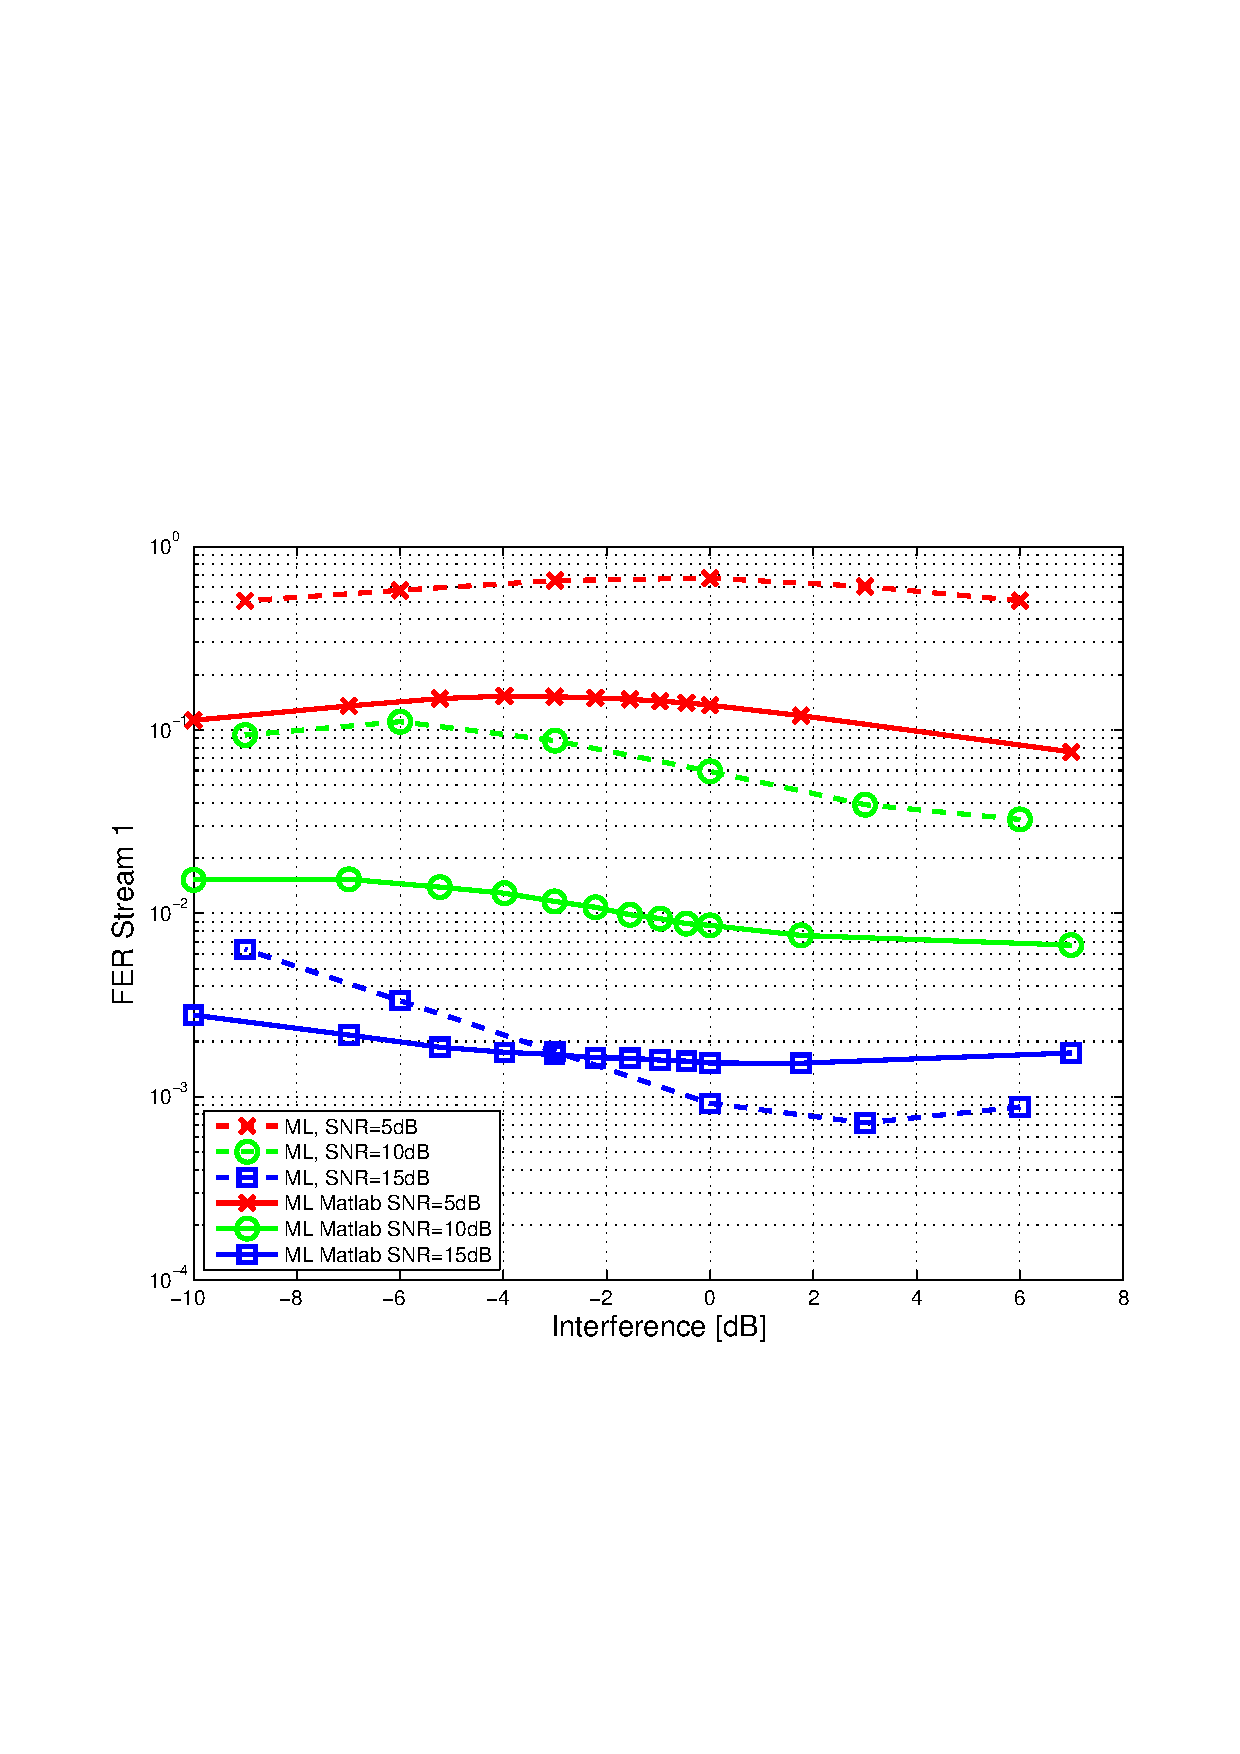
\includegraphics[width=\columnwidth]{figures/sim_results_ML_C+matlab}
 \caption{Frame error rate of the first stream of the ML receiver (C and Matlab implementation) for a frequency flat Rayleigh fading channel. Results are plotted for different SNR levels of the first stream. The $x$ axis denotes the interference of the second stream w.r.t\ the first stream.}
\label{fig:sim_results_ML}
\end{figure}

\begin{figure}
 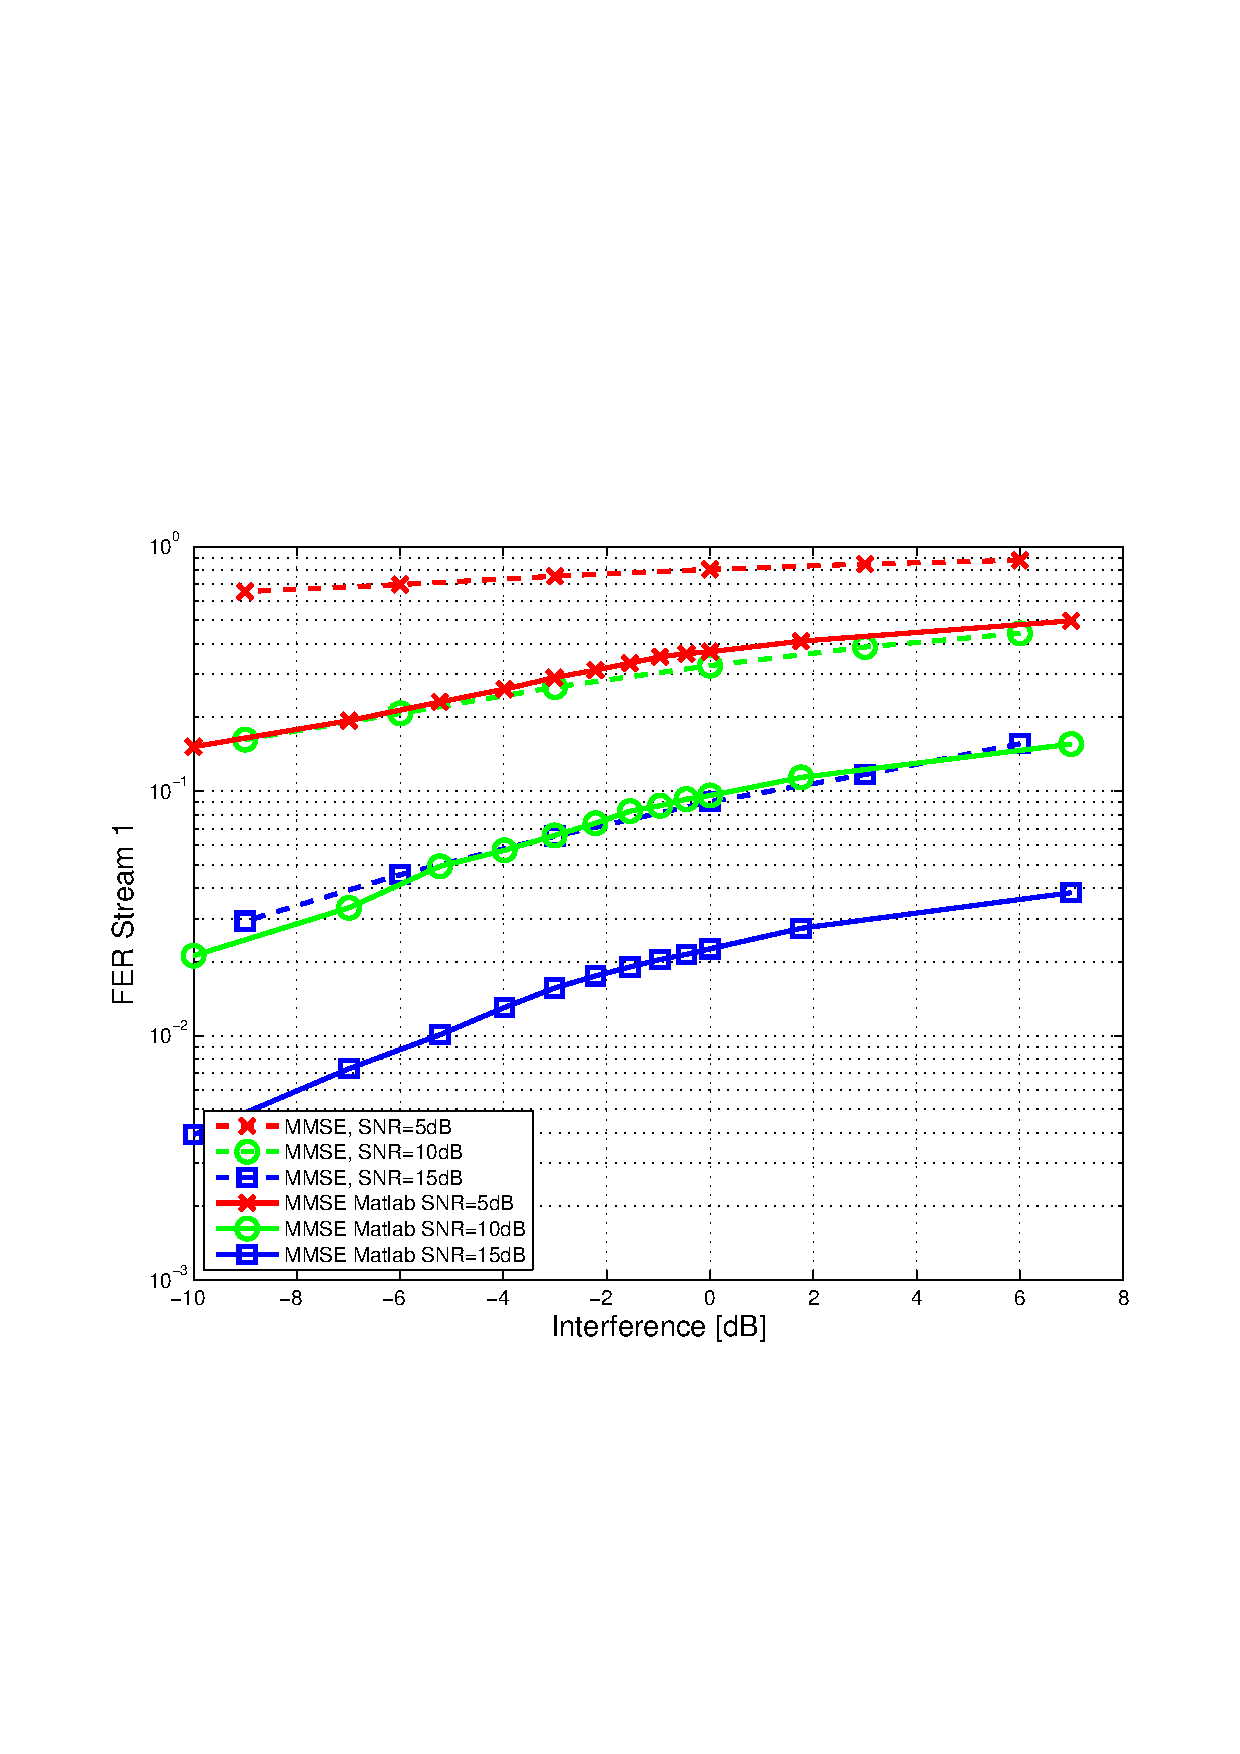
\includegraphics[width=\columnwidth]{figures/sim_results_MMSE_C+matlab}
 \caption{Frame error rate of the first stream of the MMSE receiver (C and Matlab implementation) for a frequency flat Rayleigh fading channel. Results are plotted for different SNR levels of the first stream. The $x$ axis denotes the interference of the second stream w.r.t\ the first stream.}
\label{fig:sim_results_MMSE}
\end{figure}

\begin{figure}
 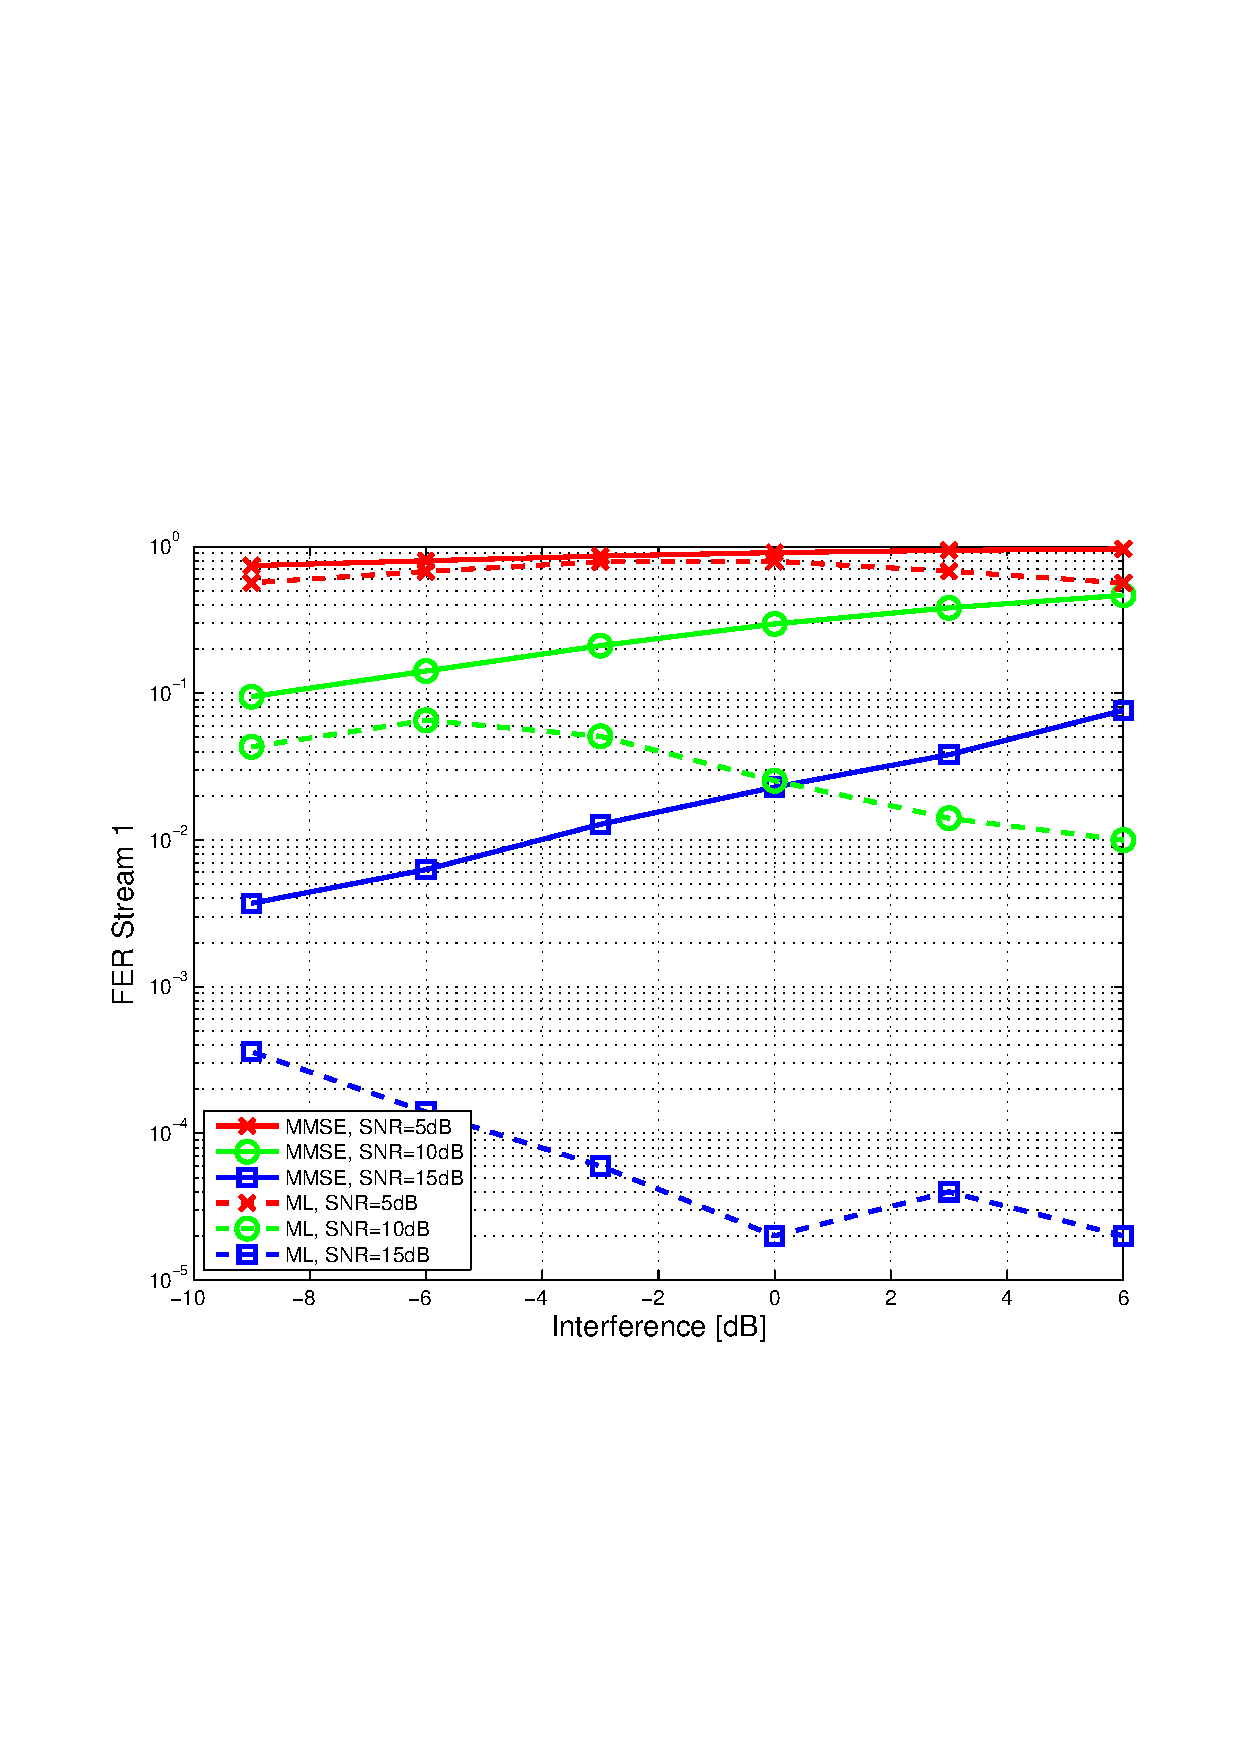
\includegraphics[width=\columnwidth]{figures/sim_results_ML+MMSE_C_freq_sel}
 \caption{Frame error rate of the first stream of the of the MMSE and ML receiver (C implementation) for a frequency selective Rayleigh fading channel. Results are plotted for different SNR levels of the first stream. The $x$ axis denotes the interference of the second stream w.r.t.\ the first stream.}
\label{fig:sim_results_MMSE+ML_freq_sel}
\end{figure}


% \begin{figure}[p]
%  \includegraphics[width=\columnwidth]{figures/results_rice10_aoa2}
%  \caption{Frame error rate of ML and MMSE receiver for a Ricean fading channel ($K=10$ dB) and a $\pi/2$ angle between culsters. Results are plotted for different SNR levels of the first stream. The $x$ axis denotes the interference of the second stream wrt the first stream.}
% \label{fig:results_rice10_aoa2}
% \end{figure}
% 
% \begin{figure}[p]
%  \includegraphics[width=\columnwidth]{figures/results_rice10_aoa4}
%  \caption{Frame error rate of ML and MMSE receiver for a Ricean fading channel ($K=10$ dB)  and a $\pi/4$ angle between culsters. Results are plotted for different SNR levels of the first stream. The $x$ axis denotes the interference of the second stream wrt the first stream.}
% \label{fig:results_rice10_aoa4}
% \end{figure}
% 
% \begin{figure}[p]
%  \includegraphics[width=\columnwidth]{figures/results_rice10_aoa8}
%  \caption{Frame error rate of ML and MMSE receiver for a Ricean fading channel ($K=10$ dB)  and a $\pi/8$ angle between culsters. Results are plotted for different SNR levels of the first stream. The $x$ axis denotes the interference of the second stream wrt the first stream.}
% \label{fig:results_rice10_aoa8}
% \end{figure}

\begin{figure}
 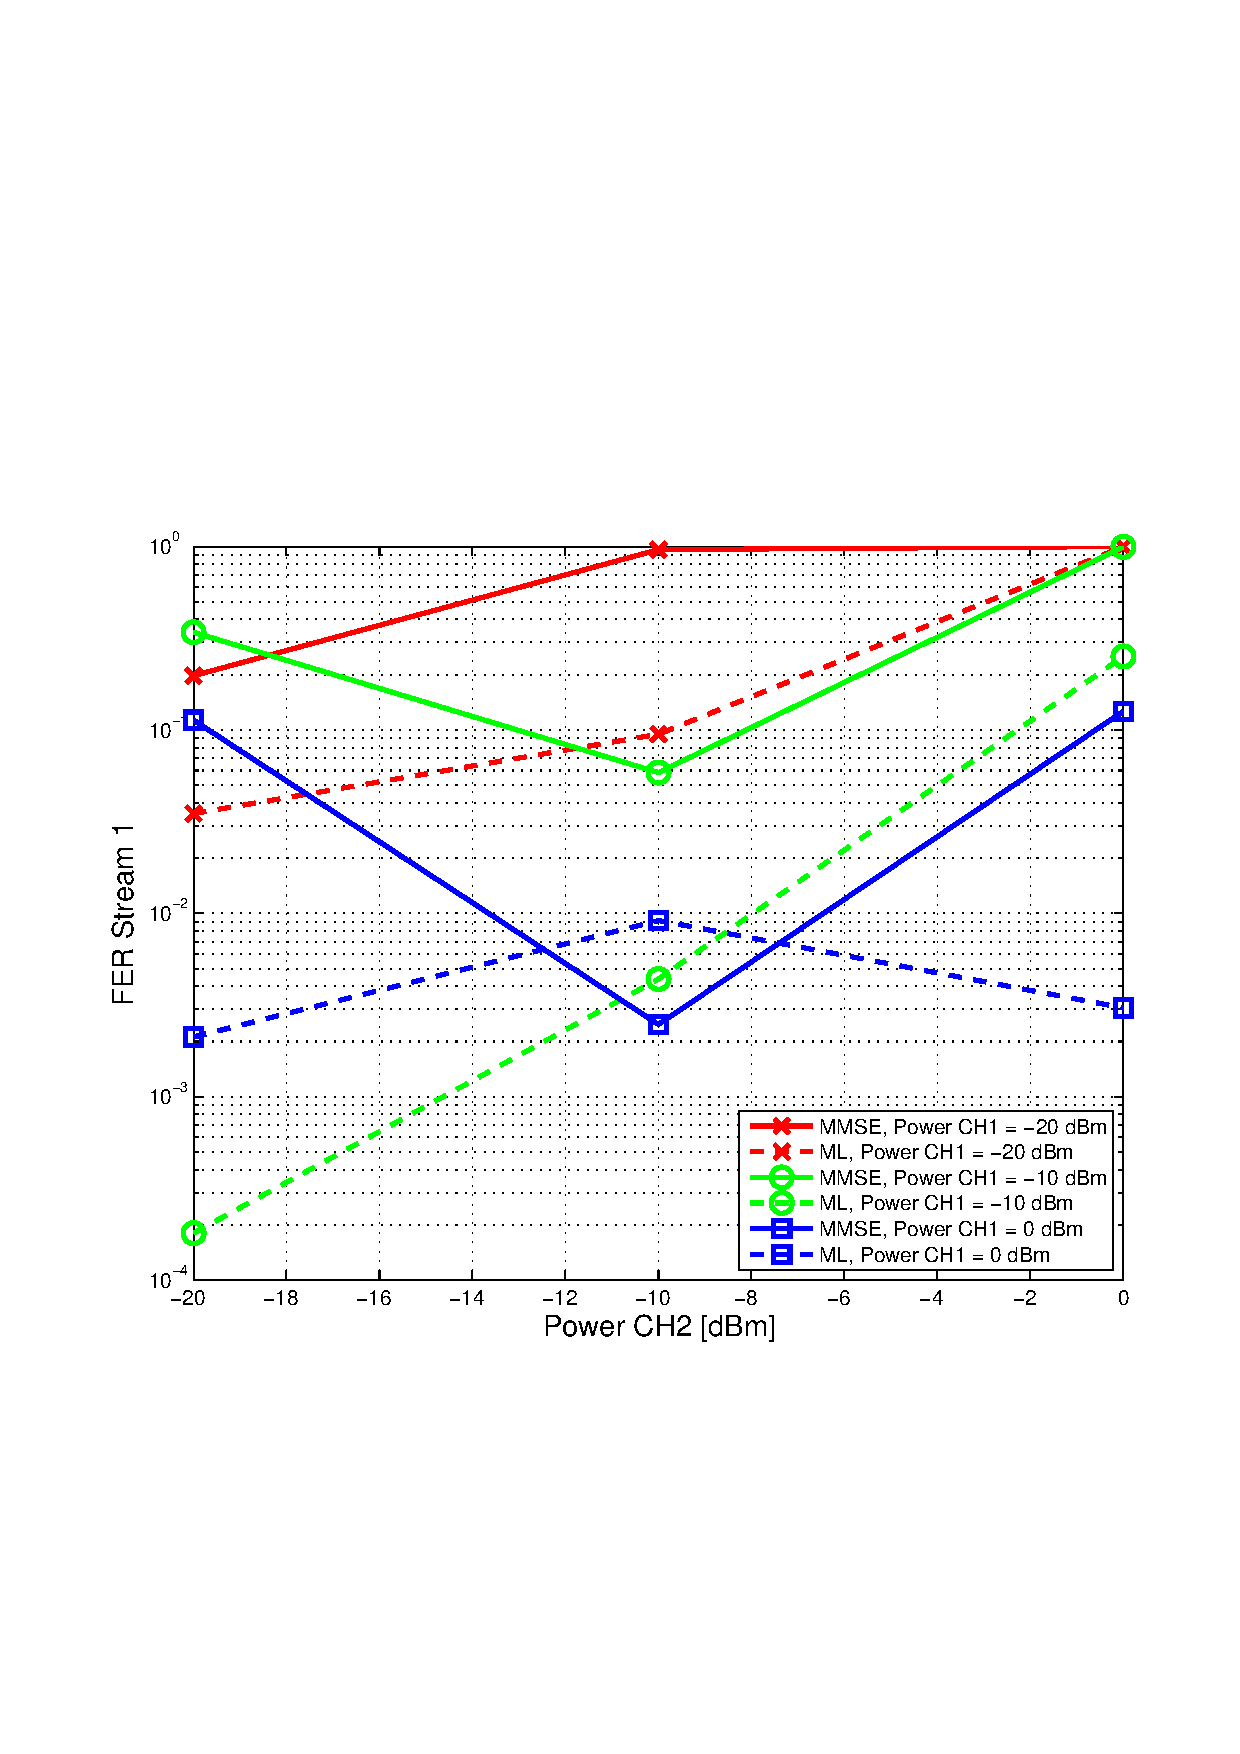
\includegraphics[width=\columnwidth]{figures/emos_results_ML+MMSE}
 \caption{Measured frame error rate of the first stream using real-time MMSE and ML receiver in the Eurecom lab. Results are plotted for different power levels of the two clusterheads.}
\label{fig:emos_results}
\end{figure}

\subsection{Lab Tests}
\label{sec:lab}

\subsubsection{Test Setup}

The dual stream receiver was tested in the lab using an extended version of the Eurecom MIMO OpenAir Sounder (EMOS) \cite{kaltenberger09}. The EMOS can be seen as a stand-alone version of the physical layer of the OpenAirMesh testbed. Only the synchronization symbols (CHSCH, MRSCH) and the broadcast channels (CHBCH, MRBCH) are transmitted. Instead of the scheduled access channels, additional pilot symbols are transmitted that can be used for channel sounding purposes, but this functionality is not used in this paper. Instead we record the frame error rates (based on the CRC check) of the CHBCH. Note that the real-time system uses the same fixed point code for the receiver as the simulator.

For the experiments we set up three nodes (CH1, CH2 and MR2) in our lab. To simulate different SNR levels at the receiver we changed the transmit powers of the two CHs between -20\,dBm and 0\,dBm. 

\subsubsection{Results}

Figure \ref{fig:emos_results} show the FER of the second stream for different SNR values for the ML, the MMSE and the single stream receiver respectively. It can be seen that the results show a very high volatility, which is mostly due to the fact of the wireless channel, which cannot be controlled as nicely as in the simulations. However, the basic trends are the same as in the simulations. It can be seen that the MMSE receiver has in general a worse performance than the ML receiver. 

% \begin{figure}
%  \includegraphics[width=\columnwidth]{figures/FER2_idx0}
%  \caption{Measured frame error rate of the second stream using ML receiver. Results are plotted for different SNR levels of the two streams.}
% \label{fig:FER2_3D_idx0}
% \end{figure}
% 
% \begin{figure}
%  \includegraphics[width=\columnwidth]{figures/FER2_idx2}
%  \caption{Measured frame error rate of the second stream using MMSE receiver. Results are plotted for different SNR levels of the two streams.}
% \label{fig:FER2_3D_idx2}
% \end{figure}
% 
% \begin{figure}
%  \includegraphics[width=\columnwidth]{figures/FER2_idx4}
%  \caption{Measured frame error rate of the second stream using single stream receiver. Results are plotted for different SNR levels of the two streams.}
% \label{fig:FER2_3D_idx4}
% \end{figure}

\begin{figure*}
 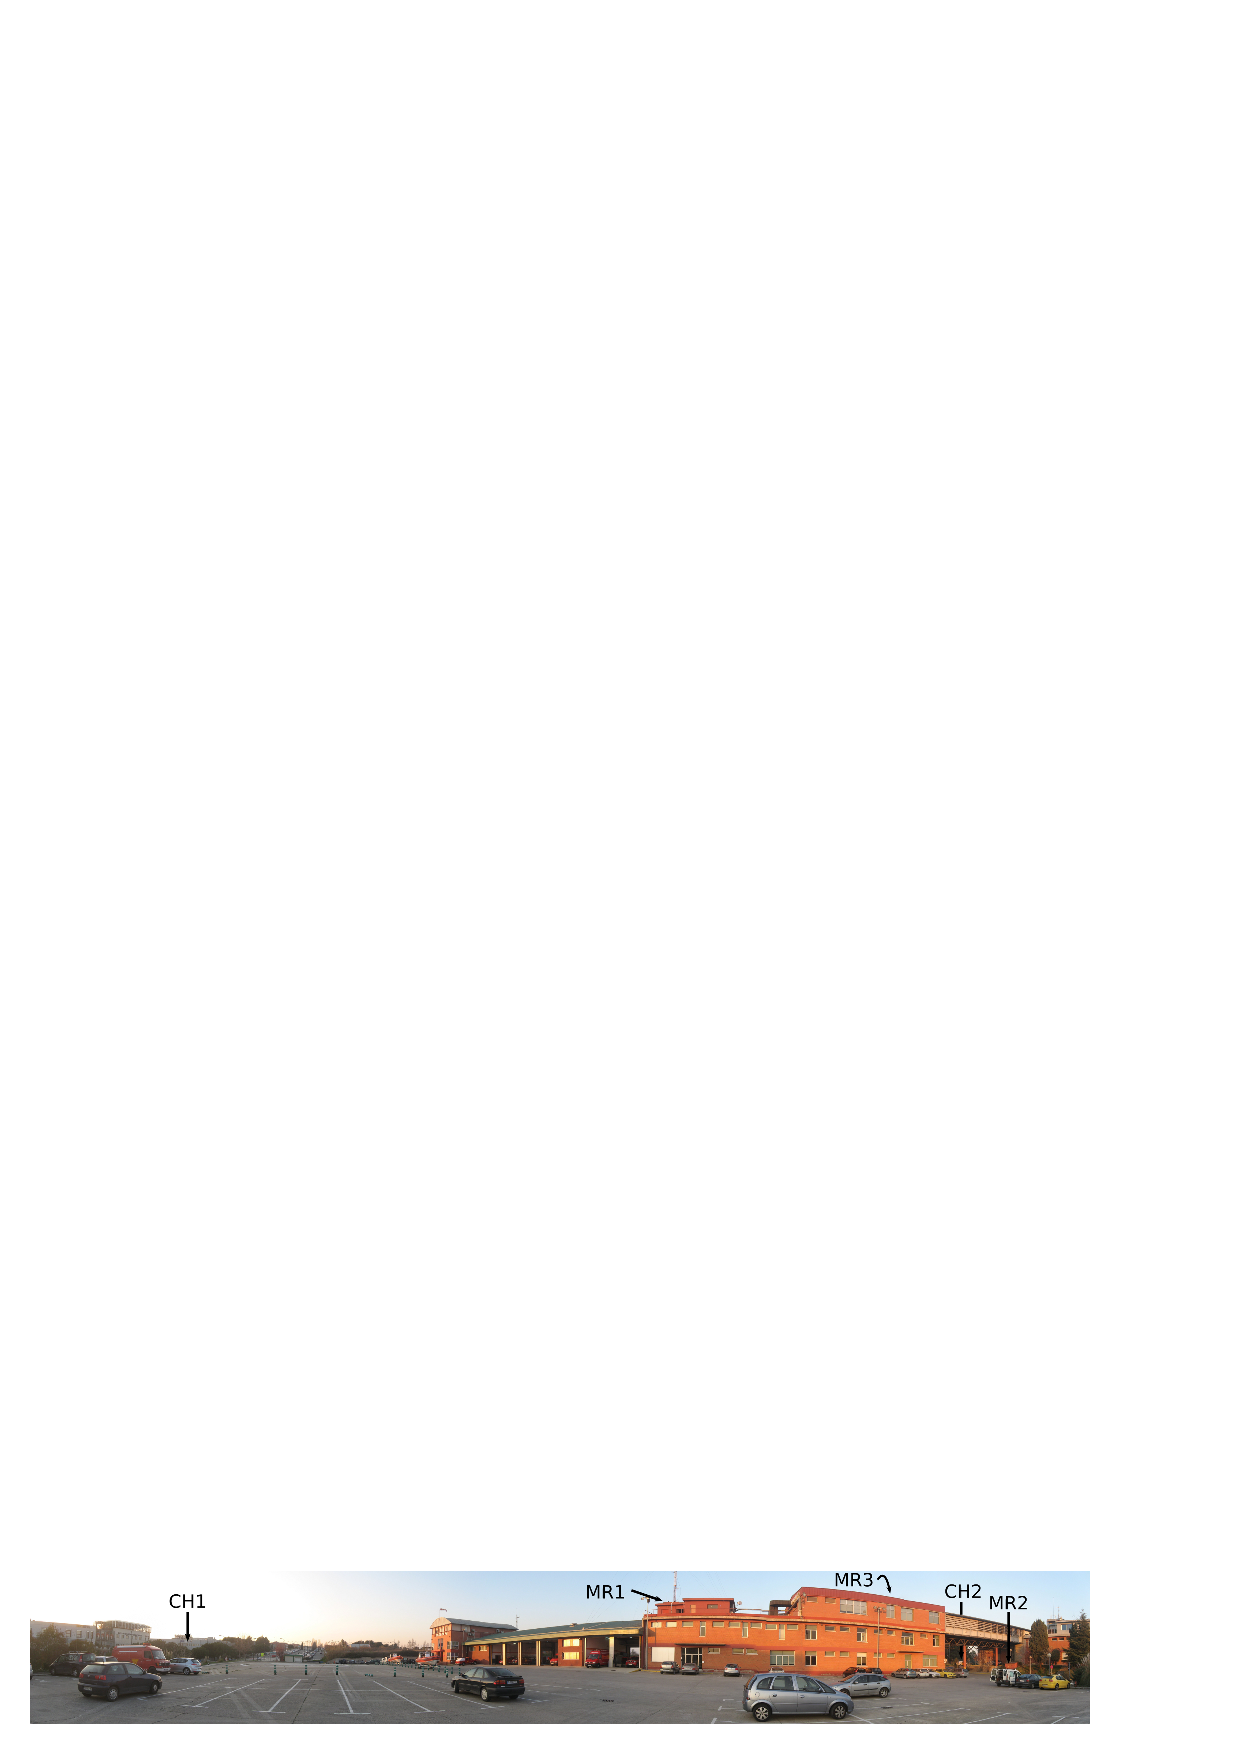
\includegraphics[width=\textwidth]{figures/pano_5nodes_annotated_300dpi}
\caption{Five node mesh network trial in Bellaterra, Spain. MR1 is located at the roof of the red fire brigade building. CH1 and MR2 are located on opposite sides of the parking lot in front of the building. CH2 and MR3 are on the other side of the building.}
\label{fig:mesh_5nodes}
\end{figure*}

\subsection{Field Trials}
\label{sec:trial}


One major application of OpenAirMesh platform is the demonstration of rapidly-deployable broadband ad hoc communications systems for public safety units in interventions following natural hazards and industrial accidents. Such a demonstration took place in February 2009 in Bellaterra, Spain in the context of the European project CHORIST, which is funded by the 6th framework program (www.chorist.eu). 

%Such public safety units require a reliable communication broadband system and services that do not need heavy management operations involvement in order to allow them to increase their efficiency during their critical interventions.  

During the trials we set up a mesh network with five node as depicted in Fig.\ \ref{fig:mesh_topology} on the parking lot of the fire brigade building in Bellaterra (see Fig.\ \ref{fig:mesh_5nodes}). MR1 was placed on the roof of the building and served as an edge router establishing the connection to the core network and the control room. CH1 and MR2 were placed on the parking lot in front of the building. CH2 and MR3 were placed behind the building, such that there was no connection between CH1 and MR3 as well as between CH2 and MR1. MR2 was in the broadcast domain of both CHs, relaying traffic between them.

Both MR2 and MR3 were used as gateways to other networks. Two different end-to-end applications were tested on the network: a video surveillance application and a push-to-talk VoIP application. During the trials we managed to establish a reliable connection (in the sense that both applications were running smoothly) between MR1 and MR3. For more details on these trials see \cite{chorist_trials}.

%Here the elements of the mesh network are routers, some of which are edge routers in the sense that they are gateways to other networks (WIFI, bluetooth, etc.). These are some of the application scenarios considered in the CHORIST FP6 project  and future HNPS Celtic project.


% \begin{figure*}
%  \includegraphics[width=\textwidth]{figures/pano_3nodes_annotated}
% \caption{3 node mesh}
% \label{fig:mesh_3nodes}
% \end{figure*}
% 

% \begin{figure}
%  \includegraphics[width=\columnwidth]{figures/pano_5nodes_2_annotated}
% \caption{5 node mesh, cluster 2}
% \label{fig:mesh_5nodes_2}
% \end{figure}

\section{Conclusions}
\label{sec:con}

In this paper we have shown the feasibility of distributed network synchronization and distributed MIMO on the real-time open-source OpenAirInterface platform. We conclude this paper by describing a few lessons we have learned during the implementation and the field trials. 

Synchronization is a prerequisite for the distributed MIMO receiver described in this paper and other cooperative communication schemes. We have seen that the proposed synchronization is feasible for small scale networks in indoor and medium-range outdoor scenarios. For larger networks, the requirement of a single reference clock is somewhat restrictive, since when it fails the whole network fails. Also it is not proven that the algorithm is stable in larger networks. We are planning to investigate this issue in future publications.

As for the implementation of the distributed MIMO receiver we have seen that the reduced complexity max-log MAP detector has several advantages over the linear MMSE receiver. First of all its performance is much better (both diversity and coding gain), especially when the interference level is high. Further it can be implemented without any divisions which is very advantageous on a fixed point processor. The implementation of the MMSE receiver on the other requires a matrix inversion, which is not trivial using fixed point arithmetic and looses a lot of accuracy.    

During the trials we have also seen that the distributed MIMO receiver is very sensitive to channel conditions. The best performance is achieved if the two transmitters have a line of sight to the receiver, but are well separated in space. Small displacements of the antennas can also make a big difference. Significant differences in the received powers form the two sources can also improve the performance (in case of the max-log MAP receiver). 

In future work we would like to include distributed space-time coding and collaborative beamforming into OpenAirInterface. This could for example be used in a multiple relay channel, when several relays are placed between two clusterheads. One particular aspect we would like to investigate are the consequences of such scenarios on design aspects related to spatial HARQ and channel coding mechanisms.

% Applications of the OpenAirMesh platform include demonstration of broadband ad hoc communications systems for public safety units as well as demonstration of collaborative communication in a cognitive radio system. 


% References should be produced using the bibtex program from suitable
% BiBTeX files (here: strings, refs). The IEEEbib.bst bibliography
% style file from IEEE produces unsorted bibliography list.
% -------------------------------------------------------------------------

%\renewcommand{\url}[1]{}
\bibliographystyle{IEEEtran}
\bibliography{IEEEabrv,OpenAirMesh}


\end{document}